% Options for packages loaded elsewhere
\PassOptionsToPackage{unicode}{hyperref}
\PassOptionsToPackage{hyphens}{url}
\PassOptionsToPackage{dvipsnames,svgnames,x11names}{xcolor}
%

\documentclass[
  a4paper, 
  twoside,
  final
]{article}

\usepackage{amsmath,amssymb}
\usepackage{iftex}
\ifPDFTeX
  \usepackage[T1]{fontenc}
  \usepackage[utf8]{inputenc}
  \usepackage{textcomp} % provide euro and other symbols
\else % if luatex or xetex
  \usepackage{unicode-math}
  \defaultfontfeatures{Scale=MatchLowercase}
  \defaultfontfeatures[\rmfamily]{Ligatures=TeX,Scale=1}
\fi
\usepackage{lmodern}
\ifPDFTeX\else  
    % xetex/luatex font selection
\fi
% Use upquote if available, for straight quotes in verbatim environments
\IfFileExists{upquote.sty}{\usepackage{upquote}}{}
\IfFileExists{microtype.sty}{% use microtype if available
  \usepackage[]{microtype}
  \UseMicrotypeSet[protrusion]{basicmath} % disable protrusion for tt fonts
}{}
\makeatletter
\@ifundefined{KOMAClassName}{% if non-KOMA class
  \IfFileExists{parskip.sty}{%
    \usepackage{parskip}
  }{% else
    \setlength{\parindent}{0pt}
    \setlength{\parskip}{6pt plus 2pt minus 1pt}}
}{% if KOMA class
  \KOMAoptions{parskip=half}}
\makeatother
\usepackage{xcolor}
\setlength{\emergencystretch}{3em} % prevent overfull lines
\setcounter{secnumdepth}{5}
% Make \paragraph and \subparagraph free-standing
\makeatletter
\ifx\paragraph\undefined\else
  \let\oldparagraph\paragraph
  \renewcommand{\paragraph}{
    \@ifstar
      \xxxParagraphStar
      \xxxParagraphNoStar
  }
  \newcommand{\xxxParagraphStar}[1]{\oldparagraph*{#1}\mbox{}}
  \newcommand{\xxxParagraphNoStar}[1]{\oldparagraph{#1}\mbox{}}
\fi
\ifx\subparagraph\undefined\else
  \let\oldsubparagraph\subparagraph
  \renewcommand{\subparagraph}{
    \@ifstar
      \xxxSubParagraphStar
      \xxxSubParagraphNoStar
  }
  \newcommand{\xxxSubParagraphStar}[1]{\oldsubparagraph*{#1}\mbox{}}
  \newcommand{\xxxSubParagraphNoStar}[1]{\oldsubparagraph{#1}\mbox{}}
\fi
\makeatother

\usepackage{color}
\usepackage{fancyvrb}
\newcommand{\VerbBar}{|}
\newcommand{\VERB}{\Verb[commandchars=\\\{\}]}
\DefineVerbatimEnvironment{Highlighting}{Verbatim}{commandchars=\\\{\}}
% Add ',fontsize=\small' for more characters per line
\usepackage{framed}
\definecolor{shadecolor}{RGB}{241,243,245}
\newenvironment{Shaded}{\begin{snugshade}}{\end{snugshade}}
\newcommand{\AlertTok}[1]{\textcolor[rgb]{0.68,0.00,0.00}{#1}}
\newcommand{\AnnotationTok}[1]{\textcolor[rgb]{0.37,0.37,0.37}{#1}}
\newcommand{\AttributeTok}[1]{\textcolor[rgb]{0.40,0.45,0.13}{#1}}
\newcommand{\BaseNTok}[1]{\textcolor[rgb]{0.68,0.00,0.00}{#1}}
\newcommand{\BuiltInTok}[1]{\textcolor[rgb]{0.00,0.23,0.31}{#1}}
\newcommand{\CharTok}[1]{\textcolor[rgb]{0.13,0.47,0.30}{#1}}
\newcommand{\CommentTok}[1]{\textcolor[rgb]{0.37,0.37,0.37}{#1}}
\newcommand{\CommentVarTok}[1]{\textcolor[rgb]{0.37,0.37,0.37}{\textit{#1}}}
\newcommand{\ConstantTok}[1]{\textcolor[rgb]{0.56,0.35,0.01}{#1}}
\newcommand{\ControlFlowTok}[1]{\textcolor[rgb]{0.00,0.23,0.31}{\textbf{#1}}}
\newcommand{\DataTypeTok}[1]{\textcolor[rgb]{0.68,0.00,0.00}{#1}}
\newcommand{\DecValTok}[1]{\textcolor[rgb]{0.68,0.00,0.00}{#1}}
\newcommand{\DocumentationTok}[1]{\textcolor[rgb]{0.37,0.37,0.37}{\textit{#1}}}
\newcommand{\ErrorTok}[1]{\textcolor[rgb]{0.68,0.00,0.00}{#1}}
\newcommand{\ExtensionTok}[1]{\textcolor[rgb]{0.00,0.23,0.31}{#1}}
\newcommand{\FloatTok}[1]{\textcolor[rgb]{0.68,0.00,0.00}{#1}}
\newcommand{\FunctionTok}[1]{\textcolor[rgb]{0.28,0.35,0.67}{#1}}
\newcommand{\ImportTok}[1]{\textcolor[rgb]{0.00,0.46,0.62}{#1}}
\newcommand{\InformationTok}[1]{\textcolor[rgb]{0.37,0.37,0.37}{#1}}
\newcommand{\KeywordTok}[1]{\textcolor[rgb]{0.00,0.23,0.31}{\textbf{#1}}}
\newcommand{\NormalTok}[1]{\textcolor[rgb]{0.00,0.23,0.31}{#1}}
\newcommand{\OperatorTok}[1]{\textcolor[rgb]{0.37,0.37,0.37}{#1}}
\newcommand{\OtherTok}[1]{\textcolor[rgb]{0.00,0.23,0.31}{#1}}
\newcommand{\PreprocessorTok}[1]{\textcolor[rgb]{0.68,0.00,0.00}{#1}}
\newcommand{\RegionMarkerTok}[1]{\textcolor[rgb]{0.00,0.23,0.31}{#1}}
\newcommand{\SpecialCharTok}[1]{\textcolor[rgb]{0.37,0.37,0.37}{#1}}
\newcommand{\SpecialStringTok}[1]{\textcolor[rgb]{0.13,0.47,0.30}{#1}}
\newcommand{\StringTok}[1]{\textcolor[rgb]{0.13,0.47,0.30}{#1}}
\newcommand{\VariableTok}[1]{\textcolor[rgb]{0.07,0.07,0.07}{#1}}
\newcommand{\VerbatimStringTok}[1]{\textcolor[rgb]{0.13,0.47,0.30}{#1}}
\newcommand{\WarningTok}[1]{\textcolor[rgb]{0.37,0.37,0.37}{\textit{#1}}}

\providecommand{\tightlist}{%
  \setlength{\itemsep}{0pt}\setlength{\parskip}{0pt}}\usepackage{longtable,booktabs,array}
\usepackage{calc} % for calculating minipage widths
% Correct order of tables after \paragraph or \subparagraph
\usepackage{etoolbox}
\makeatletter
\patchcmd\longtable{\par}{\if@noskipsec\mbox{}\fi\par}{}{}
\makeatother
% Allow footnotes in longtable head/foot
\IfFileExists{footnotehyper.sty}{\usepackage{footnotehyper}}{\usepackage{footnote}}
\makesavenoteenv{longtable}
\usepackage{graphicx}
\makeatletter
\def\maxwidth{\ifdim\Gin@nat@width>\linewidth\linewidth\else\Gin@nat@width\fi}
\def\maxheight{\ifdim\Gin@nat@height>\textheight\textheight\else\Gin@nat@height\fi}
\makeatother
% Scale images if necessary, so that they will not overflow the page
% margins by default, and it is still possible to overwrite the defaults
% using explicit options in \includegraphics[width, height, ...]{}
\setkeys{Gin}{width=\maxwidth,height=\maxheight,keepaspectratio}
% Set default figure placement to htbp
\makeatletter
\def\fps@figure{htbp}
\makeatother

\usepackage{region,hyperref,multirow}
\definecolor{mypink}{RGB}{219, 48, 122}
\makeatletter
\@ifpackageloaded{caption}{}{\usepackage{caption}}
\AtBeginDocument{%
\ifdefined\contentsname
  \renewcommand*\contentsname{Table of contents}
\else
  \newcommand\contentsname{Table of contents}
\fi
\ifdefined\listfigurename
  \renewcommand*\listfigurename{List of Figures}
\else
  \newcommand\listfigurename{List of Figures}
\fi
\ifdefined\listtablename
  \renewcommand*\listtablename{List of Tables}
\else
  \newcommand\listtablename{List of Tables}
\fi
\ifdefined\figurename
  \renewcommand*\figurename{Figure}
\else
  \newcommand\figurename{Figure}
\fi
\ifdefined\tablename
  \renewcommand*\tablename{Table}
\else
  \newcommand\tablename{Table}
\fi
}
\@ifpackageloaded{float}{}{\usepackage{float}}
\floatstyle{ruled}
\@ifundefined{c@chapter}{\newfloat{codelisting}{h}{lop}}{\newfloat{codelisting}{h}{lop}[chapter]}
\floatname{codelisting}{Listing}
\newcommand*\listoflistings{\listof{codelisting}{List of Listings}}
\makeatother
\makeatletter
\makeatother
\makeatletter
\@ifpackageloaded{caption}{}{\usepackage{caption}}
\@ifpackageloaded{subcaption}{}{\usepackage{subcaption}}
\makeatother
\makeatletter
\@ifpackageloaded{tikz}{}{\usepackage{tikz}}
\makeatother
        \newcommand*\circled[1]{\tikz[baseline=(char.base)]{
          \node[shape=circle,draw,inner sep=1pt] (char) {{\scriptsize#1}};}}  
                  

\ifLuaTeX
  \usepackage{selnolig}  % disable illegal ligatures
\fi
\usepackage[]{natbib}
\bibliographystyle{region}
\usepackage{bookmark}

\IfFileExists{xurl.sty}{\usepackage{xurl}}{} % add URL line breaks if available
\urlstyle{same} % disable monospaced font for URLs
\hypersetup{
  pdftitle={Spatial Inequality},
  pdfauthor={Sergio J. Rey},
  pdfkeywords={spatial inequality, disparities, regions},
  colorlinks=true,
  linkcolor={blue},
  filecolor={Maroon},
  citecolor={Blue},
  urlcolor={blue},
  pdfcreator={LaTeX via pandoc}}




\title{Spatial Inequality}
\author{%
Sergio J. Rey\parnote{San Diego State University, San Diego, USA}}
\date{}

\setcounter{page}{999}
\renewcommand{\thepage}{\arabic{page}}  % L for Letters, R for Resources, E for Editorial
\jvol{1} 
\jnum{1} 
\jyear{2020} 
\jpages{999--999} 
\jauthor{S.J.~Rey} 
\received{August 21, 2024} 
\accepted{} 

\jdoi{10.18335/region.v??i??.???} 

\setlength{\parskip}{0pt plus1pt}
\setlength{\parindent}{15pt}

% %\bibliographystyle{plainnat}
\bibpunct{(}{)}{,}{a}{}{,}   % % changes formatting in natbib, see http://merkel.zoneo.net/Latex/natbib.php
% % It can be moved into the package call!

%%%%%%%%%%% GM inserted %%%%%%%%%%%%%%%
\usepackage[breakable]{tcolorbox}

% prompt
\makeatletter
\newcommand{\boxspacing}{\kern\kvtcb@left@rule\kern\kvtcb@boxsep}
\makeatother
\newcommand{\prompt}[4]{
	\ttfamily\llap{{\color{#2}[#3]:\hspace{3pt}#4}}\vspace{-\baselineskip}
}

\definecolor{incolor}{HTML}{303F9F}
\definecolor{outcolor}{HTML}{D84315}
\definecolor{cellborder}{HTML}{CFCFCF}
\definecolor{cellbackground}{HTML}{F7F7F7}
\definecolor{celloutborder}{HTML}{FFAFAF}
\definecolor{celloutbackground}{HTML}{F7E7E7}

\newcounter{code}
%%%%%%%%%%%%%%%%%%%%%%%%%%%%%%%%%%%%%%%

\newenvironment{ROutput}{\definecolor{shadecolor}{HTML}{F7E7E7}\begin{snugshade}}{\end{snugshade}}
\newenvironment*{RInput}{}{}
\begin{document}
\maketitle
\begin{abstract}
The study of spatial inequality has gained prominence due to its
significant implications for both scientific research and policy-making.
This chapter explores the concepts and computational methods used to
measure spatial inequality, emphasizing a reproducible approach that
social scientists can apply to their research. The analysis focuses on
geographic income disparities at the sub-national level, using Mexico as
a case study. By examining various a-spatial and spatially explicit
approaches, the chapter highlights the complexities of measuring
inequality across places and over time. The discussion includes a review
of traditional inequality measures and introduces spatial decomposition
methods that account for the geographical distribution of income. The
findings underscore the importance of integrating spatial considerations
into inequality analysis to better understand the patterns and drivers
of regional disparities, thereby informing more effective and equitable
policy interventions.
\end{abstract}


\begin{quote}
Geographic income inequality has risen more than 40\% between 1980 and
2021.

-- \citet{u.s.departmentofcommerce2023GeographicInequality}
\end{quote}

\section{Introduction}\label{introduction}

The study of spatial, or geographical, disparities is crucial for both
scientific and policy-oriented reasons. Scientifically, understanding
these disparities allows researchers to uncover patterns and
correlations that are vital for advancing knowledge in various fields
such as economics \citep{kanbur2005SpatialInequality}, public health
\citep{debnath2024GeographicDisparities}, and environmental science
\citep{venter2023EnvironmentalJustice}. From a policy perspective,
recognizing and addressing geographical disparities is essential for
promoting social equity and economic development. A prime example is the
European Union\textquotesingle s Cohesion Policy, where the reduction of
spatial disparities between member regions takes center stage
\citep{agnieszka2019RegionalInequalities}. Additionally, understanding
spatial disparities can inform urban planning and environmental policies
to create more sustainable and resilient communities.

By bridging the gap between scientific research and policy
implementation, the study of geographical disparities helps in crafting
evidence-based strategies that promote balanced regional development,
reduce inequalities, and improve the overall quality of life.
Ultimately, this interdisciplinary approach fosters a deeper
understanding of the complex dynamics at play and supports the creation
of more inclusive and effective policies.

The field of spatial data science \citep{rey2023GeographicData} provides
tools to visualize and analyze spatial inequality. Thus, it is
well-positioned to support such interdisciplinary research. The goal of
this chapter is to introduce social scientists to the concepts and
measurement of spatial inequality. The emphasis is on adopting a
computationally focused and reproducible treatment that would allow
researchers to apply the methods introduced here to their own
investigations.

The chapter proceeds as follows. We first develop a conceptual
understanding of the measurement of spatial inequality. Next, we
describe the computational environment employed to analyze spatial
disparities. The specific case study is then introduced. We then discuss
different a-spatial approaches towards measuring inequality, followed by
a detailed exploration of spatially explicit approaches for measuring
geographical disparities. The chapter concludes with the identification
of future research areas in the field of spatial inequality.

\section{Inequality Concepts}\label{inequality-concepts}

The growing concern with inequality brings to mind Peter Drucker's
often-cited principle, ``You can't improve what you don't measure.''
Before we can address the technical challenges of measuring spatial
inequality, it is essential to first grapple with the conceptual issues
surrounding what we are measuring.

It is important to distinguish between terms that frequently appear in
the inequality literature: equality (inequality) and equity (inequity).
Equality refers to the state of being equal, particularly in status,
rights, and opportunities. In economics, this often means distributing
resources and opportunities uniformly across all individuals or groups.

Equity, conversely, involves fairness and justice in the distribution of
resources and opportunities. It considers individual needs and
circumstances, aiming to level the playing field. Therefore, although
inequality and inequity are interconnected within the context of social
justice \citep{sen2004InequalityReexamined}, they are not synonymous.

For instance, an equal distribution of resources, such as uniform per
capita expenditure on students, can create inequities by ignoring the
challenges faced by students in different contexts, such as urban versus
rural districts or advantaged versus disadvantaged neighborhoods
\citep{tine2017GrowingRural}. Conversely, some distributions are
intentionally unequal to achieve greater equity. Progressive income tax
schemes, where the tax rate increases with income, are a prime example
of this approach \citep{ledic2023TaxProgressivity}.

A closely related distinction is between equality of outcomes and
equality of opportunities. Inequality in outcomes refers to the unequal
distribution of income, wealth, and resources among individuals in a
society, which can result from factors such as luck, effort, and
inherited wealth. In contrast, inequality in opportunities focuses on
the unequal access to education, healthcare, and other essential
services that enable individuals to achieve their potential,
irrespective of their background \citep{roemer1998EqualityOpportunity}.
Studies may differ, then, in whether they measure spatial inequality in
outcomes \citep{khedmatimorasae2024SocialDeterminants} or spatial
disparities in opportunities \citep{knaap2017CartographyOpportunity}.

In addition to the distinction between inequality and inequity, and
between outcomes versus opportunities, there is much variation in the
substantive variable under focus. Income studies dominate the literature
quantitatively \citep{gaubert2021TrendsUS} and are sometimes contrasted
with studies of the inequality of wealth
\citep{suss2024GEOWEALTHUSSpatial}.\footnote{It is important to keep in
  mind that income is measured as a flow whereas wealth is a stock. This
  distinction matters in terms of the way disparities in the two
  variables are examined.} More granular studies examine disparities in
the sources of income, such as wages, as well as employment rates
\citep{overman2022SpatialDisparities}. Outside of economics, topics such
as disparities in educational outcomes
\citep{graetz2020MappingDisparities}, health outcomes
\citep{khedmatimorasae2024SocialDeterminants}, voting patterns
\citep{barber2022400Million}, among many others, are replete across the
social and life sciences.

The unit of measurement employed in inequality analysis is also an
important consideration. \citet{sala-i-martin2006WorldDistribution}
demonstrates that when using countries as the unit of analysis, the
picture that emerges is one of large and static levels of international
inequality. However, when the analysis used countries weighted by their
populations, the view is one of declining inequality over time. Later,
we shall see that this choice of weighting versus non-weighting of the
units is an important issue in spatial inequality measurement.

There is much variation across the inequality literature in the unit of
measure. Studies of personal income inequality often focus on data
recorded for individuals \citep{piketty2003IncomeInequality}. Other
studies take the household or family as the unit of analysis
\citep{brandolini2011IncomeInequality}. In both cases, the focus is on
income inequality across people. This is an essential point of departure
for our study of spatial inequality, which is where the unit of
measurement is a geographical area. In other words, in spatial
inequality analysis, the focus is inequality across places.

Still further, some studies examine the spatial distribution of personal
income inequality
\citep{partridge1998StatePatterns, frank2009InequalityGrowth}---that is,
how inequality between individuals within a state varies across states.
In the spatially oriented inequality studies, the geographical unit of
analysis can range from countries \citep{milanovic2018GlobalInequality},
to intra-national regions \citep{ganong2017WhyHas}, to cities
\citep{u.s.departmentofcommerce2023GeographicInequality}, and down to
neighborhoods \citep{nijman2020UrbanInequalities}.

A final inequality concept we need to consider is the role of time. One
question is the time unit. Is income measured per person, per year, or
is some life-time earnings, or permanent income
\citep{hall1978StochasticImplications} measure employed? A second
question pertains to whether the study of inequality is a snapshot at
one point in time or focuses on the dynamics of income distribution.

Addressing all these issues is beyond the scope of any one study. We
raise them here in order to situate the study of spatial inequality in a
much broader context. For this chapter, we will hone in on the question
of measuring spatial income inequality at the sub-national scale.

\section{Computational Environment}\label{computational-environment}

In the following section, we present the packages and computational
environment used. The narrative following code cells explains the
computational concepts.

\subsection{Packages}\label{packages}

\phantomsection\label{annotated-cell-1}%
\begin{Shaded}
\begin{Highlighting}[]
\ImportTok{import}\NormalTok{ inequality }\ImportTok{as}\NormalTok{ ineq }\hspace*{\fill}\NormalTok{\circled{1}}
\ImportTok{import}\NormalTok{ numpy }\ImportTok{as}\NormalTok{ np }\hspace*{\fill}\NormalTok{\circled{2}}
\ImportTok{import}\NormalTok{ pandas }\ImportTok{as}\NormalTok{ pd}
\ImportTok{import}\NormalTok{ geopandas }\ImportTok{as}\NormalTok{ gpd}
\ImportTok{import}\NormalTok{ libpysal }\ImportTok{as}\NormalTok{ lps}
\ImportTok{import}\NormalTok{ seaborn }\ImportTok{as}\NormalTok{ sns}
\ImportTok{import}\NormalTok{ matplotlib.pyplot }\ImportTok{as}\NormalTok{ plt}
\ImportTok{import}\NormalTok{ watermark}
\OperatorTok{\%}\NormalTok{load\_ext watermark}
\OperatorTok{\%}\NormalTok{watermark }\OperatorTok{{-}}\NormalTok{a }\StringTok{"Sergio Rey"} \OperatorTok{{-}}\NormalTok{u }\OperatorTok{{-}}\NormalTok{n }\OperatorTok{{-}}\NormalTok{t }\OperatorTok{{-}}\NormalTok{v }\OperatorTok{\textbackslash{}}
    \OperatorTok{{-}}\NormalTok{p numpy,pandas,scipy,matplotlib,inequality,seaborn,libpysal}
\end{Highlighting}
\end{Shaded}

\begin{description}
\tightlist
\item[\circled{1}]
We alias the package \texttt{inequality} as \texttt{ineq}
\item[\circled{2}]
We do the same for \texttt{numpy}
\end{description}

\begin{verbatim}
Author: Sergio Rey

Last updated: Wed Aug 21 2024 10:55:24

Python implementation: CPython
Python version       : 3.12.4
IPython version      : 8.26.0

numpy     : 2.0.1
pandas    : 2.2.2
scipy     : 1.14.0
matplotlib: 3.9.1
inequality: 0.1.dev170+gd70b5c0.d20240820
seaborn   : 0.13.2
libpysal  : 4.12.0
\end{verbatim}

Our analysis of spatial inequality utilizes packages from the Python
Spatial Analysis Library (\texttt{pysal}) \citep{rey2022PySALEcosystem},
together with \texttt{geopandas} \citep{jordahl2019GeopandasGeopandas}
and \texttt{seaborn} \citep{waskom2021SeabornStatistical}. The main
package focusing on measuring spatial disparities is
\texttt{inequality}, which implements analytics for measuring a-spatial
inequality and spatially explicit inequality measures. Also, from
\texttt{pysal}, we will depend on the \texttt{libpysal} package for
constructing spatial weights that are central to the analysis of spatial
inequality. \texttt{geopandas} provides for spatial data processing and
producing maps of the spatial distribution of income, while we adopt
\texttt{seaborn} for constructing a-spatial graphical views of
inequality.

For purposes of reproducibility, we include the \texttt{watermark}
package which reports the version numbers of each of the packages we use
in our analysis.

\section{Data}\label{data}

To illustrate the core concepts in spatial inequality measurement, we
will rely on a data set for the states in Mexico
\citep{rey2010InterregionalInequality}. The variable of interest is
state per capita gross domestic product measured in 2000 USD measured
for each decade from 1940-2000 for each of 32 areas consisting of the 31
federal states of Mexico plus Mexico City. This data-set is included as
an example data-set in \texttt{libpysal}.

\begin{Shaded}
\begin{Highlighting}[]
\NormalTok{lps.examples.explain(}\StringTok{"mexico"}\NormalTok{)}
\end{Highlighting}
\end{Shaded}

\begin{verbatim}
mexico
======

Decennial per capita incomes of Mexican states 1940-2000
--------------------------------------------------------

* mexico.csv: attribute data. (n=32, k=13)
* mexico.gal: spatial weights in GAL format.
* mexicojoin.shp: Polygon shapefile. (n=32)

Data used in Rey, S.J. and M.L. Sastre Gutierrez. (2010) "Interregional inequality dynamics in Mexico." Spatial Economic Analysis, 5: 277-298.
\end{verbatim}

In addition to the income data contained in the \texttt{mexico.csv}
file, there are two additional files available in this example:
\texttt{mexico.gal} which stores information about the contiguity
relationships between the states, and \texttt{mexicojoin.shp} which is a
shapefile.

Figure~\ref{fig-states} lists the locations of the 32 Mexican
states.\footnote{The python code used to construct this map is hidden.}

\begin{figure}

\centering{

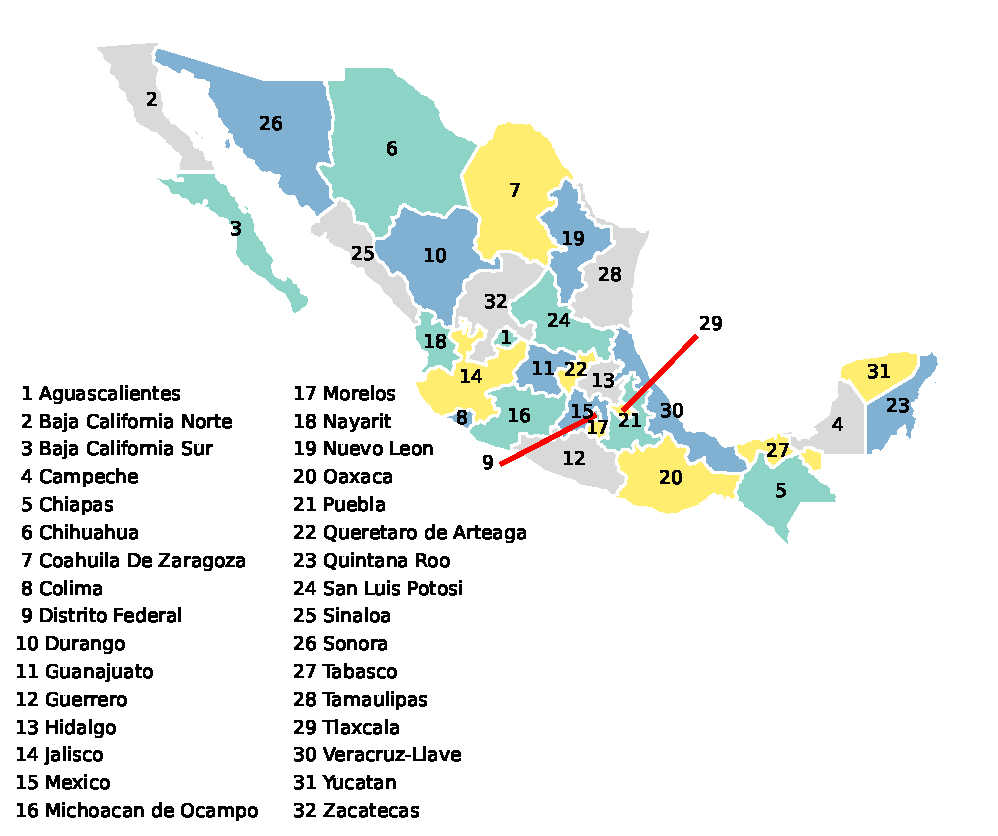
\includegraphics{spatial_inequality_files/figure-pdf/fig-states-output-1.pdf}

}

\caption{\label{fig-states}States of Mexico}

\end{figure}%

\begin{Shaded}
\begin{Highlighting}[]
\NormalTok{pth }\OperatorTok{=}\NormalTok{ lps.examples.get\_path(}\StringTok{"mexico.csv"}\NormalTok{)}
\NormalTok{df }\OperatorTok{=}\NormalTok{ pd.read\_csv(pth)}
\BuiltInTok{print}\NormalTok{(}\SpecialStringTok{f"Shape of dataframe: }\SpecialCharTok{\{}\NormalTok{df}\SpecialCharTok{.}\NormalTok{shape}\SpecialCharTok{\}}\SpecialStringTok{"}\NormalTok{)}
\BuiltInTok{print}\NormalTok{(}\SpecialStringTok{f"First 5 rows of dataframe:}\CharTok{\textbackslash{}n}\SpecialStringTok{ }\SpecialCharTok{\{}\NormalTok{df}\SpecialCharTok{.}\NormalTok{head()}\SpecialCharTok{\}}\SpecialStringTok{"}\NormalTok{)}
\NormalTok{df.head()}
\BuiltInTok{print}\NormalTok{(}\SpecialStringTok{f"}\CharTok{\textbackslash{}n}\SpecialStringTok{Variables: }\SpecialCharTok{\{}\NormalTok{df}\SpecialCharTok{.}\NormalTok{columns}\SpecialCharTok{\}}\SpecialStringTok{"}\NormalTok{)}
\end{Highlighting}
\end{Shaded}

\begin{verbatim}
Shape of dataframe: (32, 13)
First 5 rows of dataframe:
                  State  pcgdp1940  pcgdp1950  pcgdp1960  pcgdp1970  pcgdp1980  \
0       Aguascalientes    10384.0     6234.0     8714.0    16078.0    21022.0   
1      Baja California    22361.0    20977.0    17865.0    25321.0    29283.0   
2  Baja California Sur     9573.0    16013.0    16707.0    24384.0    29038.0   
3             Campeche     3758.0     4929.0     5925.0    10274.0    12166.0   
4              Chiapas     2934.0     4138.0     5280.0     7015.0    16200.0   

   pcgdp1990  pcgdp2000  hanson03  hanson98  esquivel99  inegi  inegi2  
0    20787.0    27782.0       2.0       2.0         3.0    4.0     4.0  
1    26839.0    29855.0       1.0       1.0         5.0    1.0     1.0  
2    25842.0    26103.0       2.0       2.0         6.0    1.0     1.0  
3    51123.0    36163.0       6.0       5.0         4.0    5.0     5.0  
4     8637.0     8684.0       5.0       5.0         7.0    5.0     5.0  

Variables: Index(['State', 'pcgdp1940', 'pcgdp1950', 'pcgdp1960', 'pcgdp1970',
       'pcgdp1980', 'pcgdp1990', 'pcgdp2000', 'hanson03', 'hanson98',
       'esquivel99', 'inegi', 'inegi2'],
      dtype='object')
\end{verbatim}

We can read the \texttt{mexico.csv} file using \texttt{pandas} to create
a \texttt{DataFrame} that will hold the attributes of interest. This
dataframe has the shape \texttt{(32,13)} indicating there are 32
observations on 13 variables. The 13 variables include the per capita
gross domestic product for each decade, for example \texttt{pcgdp1990}
for 1990, together with the state name, and six variables that define
different regionalization schemes for the country. We will return to
these regional variables in a later section.

\section{Measuring Spatial Inequality in
Mexico}\label{measuring-spatial-inequality-in-mexico}

\subsection{Visualizing Inequality in
Distributions}\label{visualizing-inequality-in-distributions}

We begin with different perspectives on the distribution of state
incomes in Mexico. From a geographical perspective,
Figure~\ref{fig-mappcgdp2000} shows the spatial distribution of incomes
for the last year of the sample (2000).

\begin{Shaded}
\begin{Highlighting}[]
\NormalTok{pth }\OperatorTok{=}\NormalTok{ lps.examples.get\_path(}\StringTok{"mexicojoin.shp"}\NormalTok{)}
\NormalTok{gdf }\OperatorTok{=}\NormalTok{ gpd.read\_file(pth)}
\NormalTok{ax }\OperatorTok{=}\NormalTok{ gdf.plot(column}\OperatorTok{=}\StringTok{"PCGDP2000"}\NormalTok{, k}\OperatorTok{=}\DecValTok{5}\NormalTok{, scheme}\OperatorTok{=}\StringTok{"Quantiles"}\NormalTok{,}
\NormalTok{              legend}\OperatorTok{=}\VariableTok{True}\NormalTok{,}
\NormalTok{              edgecolor}\OperatorTok{=}\StringTok{\textquotesingle{}grey\textquotesingle{}}\NormalTok{,}
\NormalTok{              legend\_kwds}\OperatorTok{=}\NormalTok{\{}\StringTok{"loc"}\NormalTok{: }\StringTok{"center left"}\NormalTok{,}
                           \StringTok{"bbox\_to\_anchor"}\NormalTok{: (}\DecValTok{1}\NormalTok{, }\FloatTok{0.5}\NormalTok{),}
                           \StringTok{"fmt"}\NormalTok{: }\StringTok{"}\SpecialCharTok{\{:.0f\}}\StringTok{"}\NormalTok{\})}
\NormalTok{ax.set\_axis\_off()}
\NormalTok{ax.set\_title(}\StringTok{"PC GDP 2000"}\NormalTok{)}\OperatorTok{;}
\end{Highlighting}
\end{Shaded}

\begin{figure}[H]

\centering{

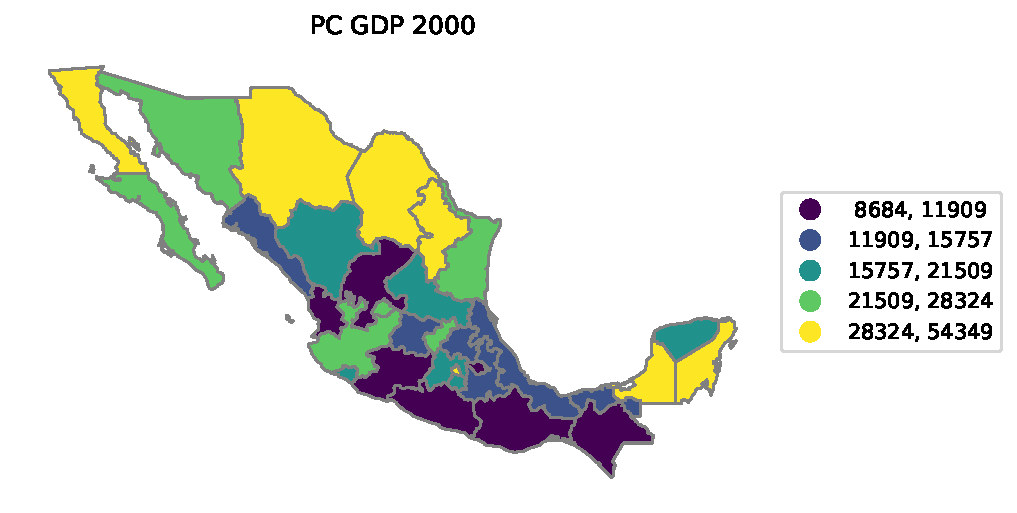
\includegraphics{spatial_inequality_files/figure-pdf/fig-mappcgdp2000-output-1.pdf}

}

\caption{\label{fig-mappcgdp2000}Per Capita Gross Domestic Product by
State (Quintiles)}

\end{figure}%

This is a choropleth map using quintiles to classify the incomes. The
visual impression is that incomes are not randomly distributed in
Mexico, as the states with incomes below the bottom quintile are more
concentrated in the south, while in the north, the highest income states
dominate. We will be able to make more quantitative evaluation of this
spatial pattern later on in this chapter.

Figure~\ref{fig-pen2000} presents a different perspective on income
distribution based on the concept of Pen's Parade, introduced by Dutch
economist Jan Pen \citep{pen1971IncomeDistribution}. The metaphor uses a
Parade to illustrate economic inequality, with each person representing
a state in the economy, and their height being proportional to the
state's per capita income. The Parade starts with the shortest
individuals depicting the poorest states, gradually increasing in height
as income rises. At the end of the parade, the tallest individuals
represent the most affluent states, highlighting the significant income
disparities across states. This visual tool showcases the inequality in
income distribution. The parade uses two different scales, with the
x-axis showing the ordinal distances between states and the y-axis
representing the interval distances in their per capita incomes.

\begin{Shaded}
\begin{Highlighting}[]
\ImportTok{from}\NormalTok{ inequality.pen }\ImportTok{import}\NormalTok{ pen}
\NormalTok{f }\OperatorTok{=}\NormalTok{ pen(gdf, }\StringTok{\textquotesingle{}PCGDP2000\textquotesingle{}}\NormalTok{, }\StringTok{\textquotesingle{}NAME\textquotesingle{}}\NormalTok{)}
\end{Highlighting}
\end{Shaded}

\begin{figure}[H]

\centering{

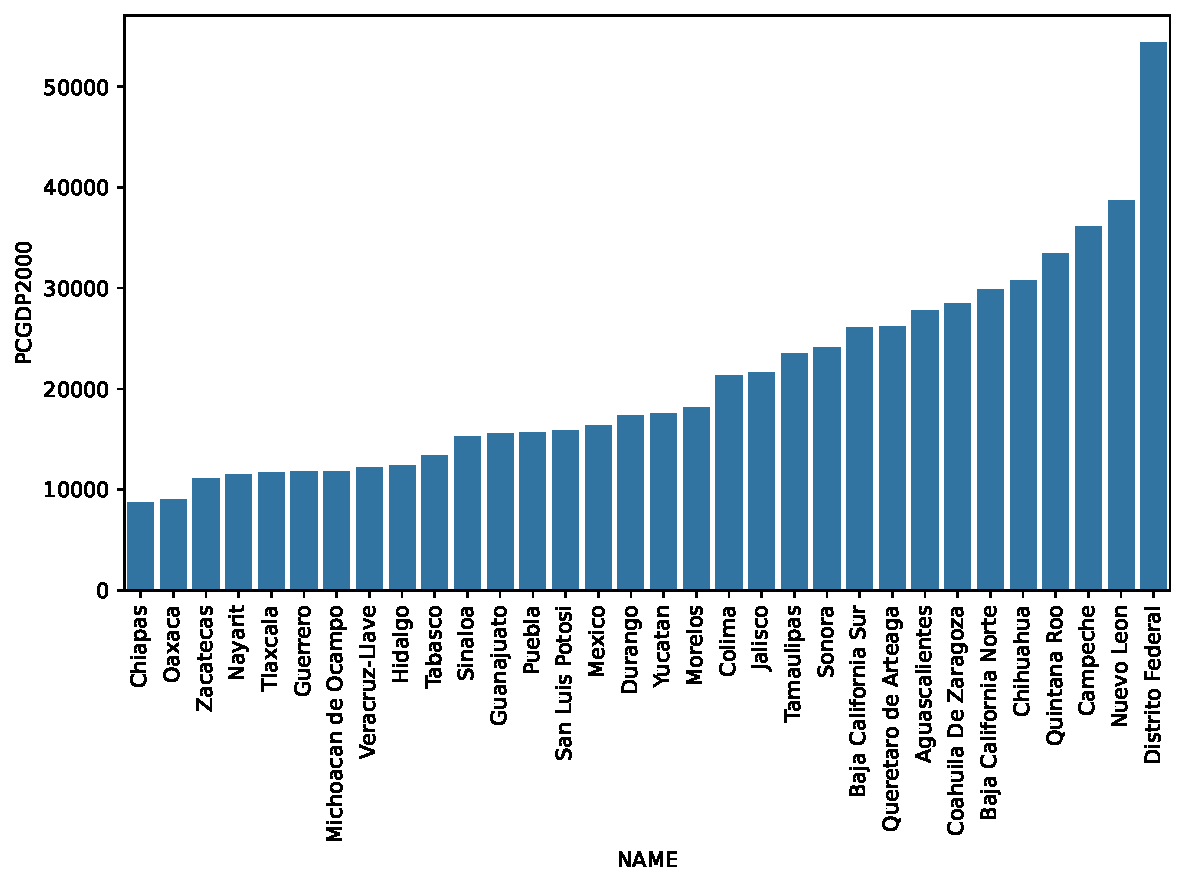
\includegraphics{spatial_inequality_files/figure-pdf/fig-pen2000-output-1.pdf}

}

\caption{\label{fig-pen2000}Pen's Parade Per Capita Gross Domestic
Product by State 2000}

\end{figure}%

We can start to integrate the spatial and attribute distributions
together using a \texttt{pengram} from the \texttt{pysal-inequality}
package:

\begin{Shaded}
\begin{Highlighting}[]
\ImportTok{from}\NormalTok{ inequality.pen }\ImportTok{import}\NormalTok{ pengram}
\NormalTok{f }\OperatorTok{=}\NormalTok{ pengram(gdf, }\StringTok{\textquotesingle{}PCGDP2000\textquotesingle{}}\NormalTok{, }\StringTok{\textquotesingle{}NAME\textquotesingle{}}\NormalTok{, xticks}\OperatorTok{=}\VariableTok{False}\NormalTok{, leg\_pos}\OperatorTok{=}\StringTok{\textquotesingle{}lower left\textquotesingle{}}\NormalTok{,}
\NormalTok{        fmt}\OperatorTok{=}\StringTok{"}\SpecialCharTok{\{:.0f\}}\StringTok{"}\NormalTok{)}
\end{Highlighting}
\end{Shaded}

\begin{figure}[H]

\centering{

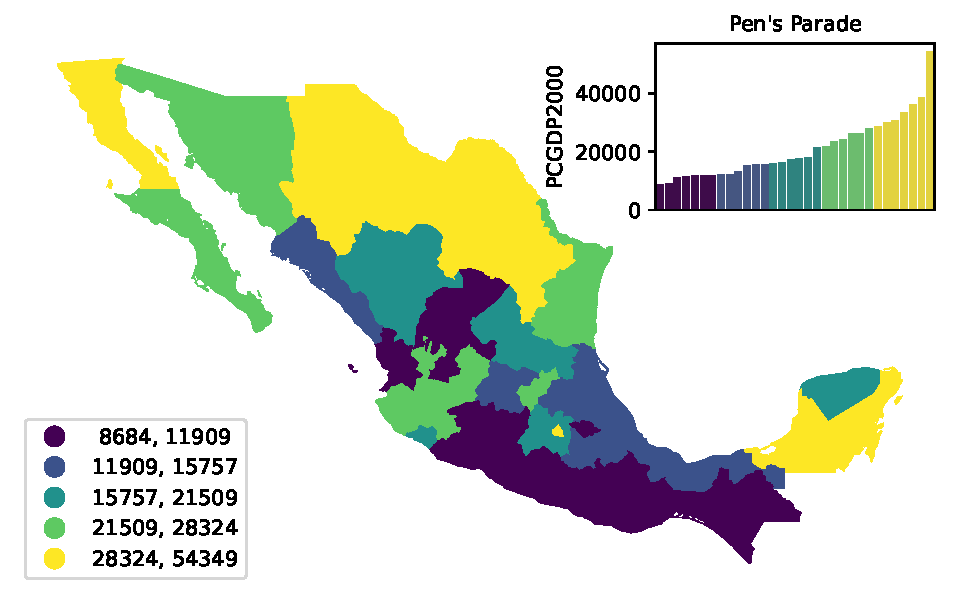
\includegraphics{spatial_inequality_files/figure-pdf/fig-pengram2000-output-1.pdf}

}

\caption{\label{fig-pengram2000}Pengram Per Capita Gross Domestic
Product by State 2000}

\end{figure}%

As shown in Figure~\ref{fig-pengram2000}, the \texttt{pengram} combines
the Pen's Parade alongside the choropleth map. This affords a more
granular view of the distribution than those offered by either view in
isolation. For example, one of the well-known limitations of a quintile
classed map is that the intra-class variation is obscured. In the
\texttt{pengram}, the intra-class variation now becomes visible through
the Pen's Parade, revealing the much larger absolute and relative
variance above the upper quintile relative to the other classes.

A second feature of the \texttt{pengram} is the ability to query for
specific observations. This makes it possible to locate the position of
a state in both the Pen's Parade (attribute space) as well as on the map
(geographical space). We do this for states occupying the two extremes
of the attribute distribution: Chiapas and Distrito Federal in
Figure~\ref{fig-pengramquery}. While the two reside in the extremes of
the attribute distribution, the high income Distrito Federal is in the
center of the geographic distribution while Chiapas is on the southern
border of the country. Moreover, although Distrito Federal stands out in
the Pen's Parade, its small geographic area makes it difficult to
identify on the map without the query functionality of the pengram.

\begin{Shaded}
\begin{Highlighting}[]
\ImportTok{from}\NormalTok{ inequality.pen }\ImportTok{import}\NormalTok{ pengram}
\NormalTok{f }\OperatorTok{=}\NormalTok{ pengram(gdf, }\StringTok{\textquotesingle{}PCGDP2000\textquotesingle{}}\NormalTok{, }\StringTok{\textquotesingle{}NAME\textquotesingle{}}\NormalTok{,  leg\_pos}\OperatorTok{=}\StringTok{\textquotesingle{}lower left\textquotesingle{}}\NormalTok{,}
\NormalTok{            fmt}\OperatorTok{=}\StringTok{"}\SpecialCharTok{\{:.0f\}}\StringTok{"}\NormalTok{,}
\NormalTok{            xticks}\OperatorTok{=}\VariableTok{False}\NormalTok{,}
\NormalTok{            query}\OperatorTok{=}\NormalTok{[}\StringTok{\textquotesingle{}Chiapas\textquotesingle{}}\NormalTok{, }\StringTok{\textquotesingle{}Distrito Federal\textquotesingle{}}\NormalTok{])}
\end{Highlighting}
\end{Shaded}

\begin{figure}[H]

\centering{

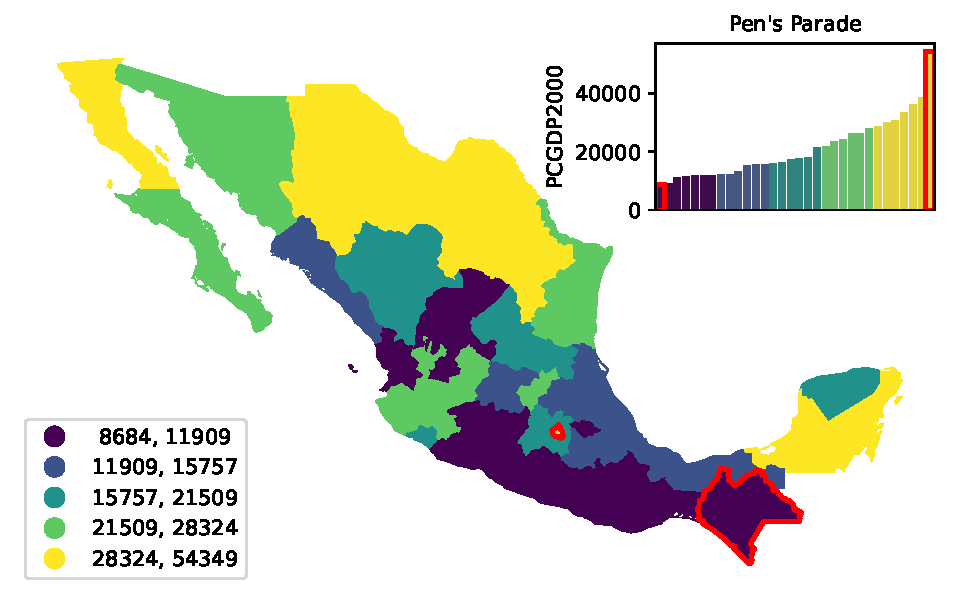
\includegraphics{spatial_inequality_files/figure-pdf/fig-pengramquery-output-1.pdf}

}

\caption{\label{fig-pengramquery}Querying the Pengram of Per Capita
Gross Domestic Product by State 2000}

\end{figure}%

Returning to a more granular view of the attribute distribution,
Figure~\ref{fig-kde2000} combines a histogram of the distribution
together with a kernel density estimate, and a rug plot. The latter
signifies the positions of each state as short ticks on the x-axis. The
outlier nature of the Distrito Federal that we saw in the
\texttt{pengram} is responsible for the positive (right) skew of the
density function. There is some evidence of polarization in the
distribution with the mode being at the poorest group of states and
other, lower, peaks in the middle of the distribution.

\begin{Shaded}
\begin{Highlighting}[]
\NormalTok{years }\OperatorTok{=} \BuiltInTok{range}\NormalTok{(}\DecValTok{1940}\NormalTok{, }\DecValTok{2010}\NormalTok{, }\DecValTok{10}\NormalTok{)}
\NormalTok{yvars }\OperatorTok{=}\NormalTok{ [}\SpecialStringTok{f\textquotesingle{}pcgdp}\SpecialCharTok{\{}\NormalTok{year}\SpecialCharTok{\}}\SpecialStringTok{\textquotesingle{}} \ControlFlowTok{for}\NormalTok{ year }\KeywordTok{in}\NormalTok{ years]}
\NormalTok{sns.histplot(df[yvars[}\OperatorTok{{-}}\DecValTok{1}\NormalTok{]], kde}\OperatorTok{=}\VariableTok{True}\NormalTok{, element}\OperatorTok{=}\StringTok{"step"}\NormalTok{,}
\NormalTok{             bins}\OperatorTok{=}\DecValTok{10}\NormalTok{, edgecolor}\OperatorTok{=}\StringTok{"black"}\NormalTok{)}
\NormalTok{sns.rugplot(df[yvars[}\OperatorTok{{-}}\DecValTok{1}\NormalTok{]], color}\OperatorTok{=}\StringTok{\textquotesingle{}blue\textquotesingle{}}\NormalTok{)}
\NormalTok{plt.show()}
\end{Highlighting}
\end{Shaded}

\begin{figure}[H]

\centering{

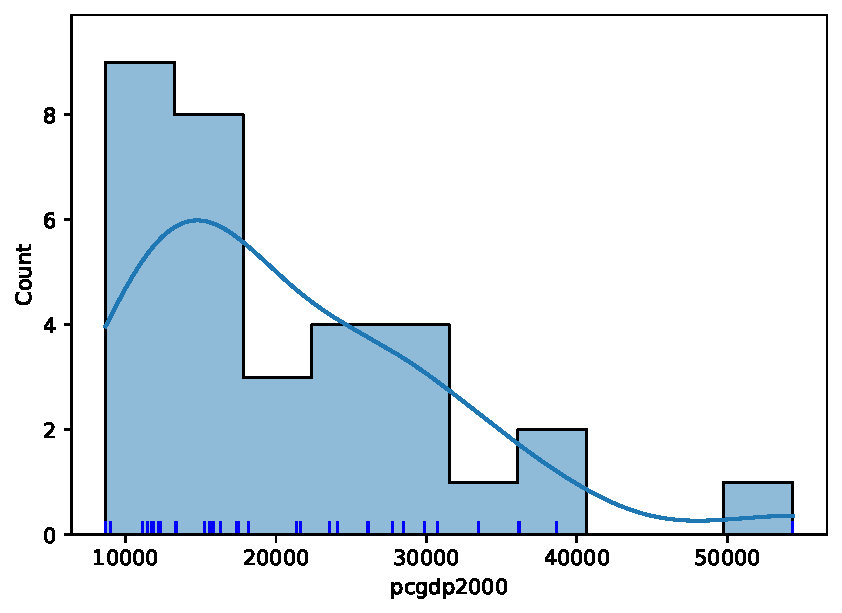
\includegraphics{spatial_inequality_files/figure-pdf/fig-kde2000-output-1.pdf}

}

\caption{\label{fig-kde2000}Distribution Per Capita Gross Domestic
Product by State 2000, histogram, kernel density, rug plot}

\end{figure}%

Inequality in a distribution is often considered by an inspection of the
shares of overall income belonging to units at different locations
within the distribution. Here, we must keep in mind, the distinction
between the different units under study in the analysis of spatial
versus personal income inequality. In spatial inequality analysis, we
essentially treat each state as an ``individual'' and set that
individual's level of income to the state's per capita income. The share
for the state is then derived as the ratio of its per capita income to
the sum of the per capita income of all states.

These shares can be portrayed in a Lorenz curve, shown in
Figure~\ref{fig-schutz2000}, which orders the states by their per capita
incomes from lowest to highest. Then, against the cumulative proportion
of states (x-axis) we plot the cumulative income share on the y-axis.
Both scales have limits of \([0, 1]\). In the case of perfect equality,
where all state per capita incomes are equal, this plot would be a
45-degree line, the so called line of perfect equality. Any departure
from perfect equality will result in states with above average per
capita income receiving more than \(1/n\) share of \(n \bar{y}\), while
states with below average per capita incomes will have shares below
\(1/n\).\footnote{States with shares below \(1/n\) would also have
  location quotients of less than one for their relative per capita
  incomes, where their per capita income was expressed relative to
  national per capita income.}

\begin{Shaded}
\begin{Highlighting}[]
\ImportTok{from}\NormalTok{ inequality.schutz }\ImportTok{import}\NormalTok{ Schutz}
\NormalTok{s }\OperatorTok{=}\NormalTok{ Schutz(gdf, }\StringTok{\textquotesingle{}PCGDP2000\textquotesingle{}}\NormalTok{)}
\NormalTok{s.plot(xlabel}\OperatorTok{=}\StringTok{\textquotesingle{}Share of States\textquotesingle{}}\NormalTok{, ylabel}\OperatorTok{=}\StringTok{\textquotesingle{}Share of Per Capita Income\textquotesingle{}}\NormalTok{)}
\end{Highlighting}
\end{Shaded}

\begin{figure}[H]

\centering{

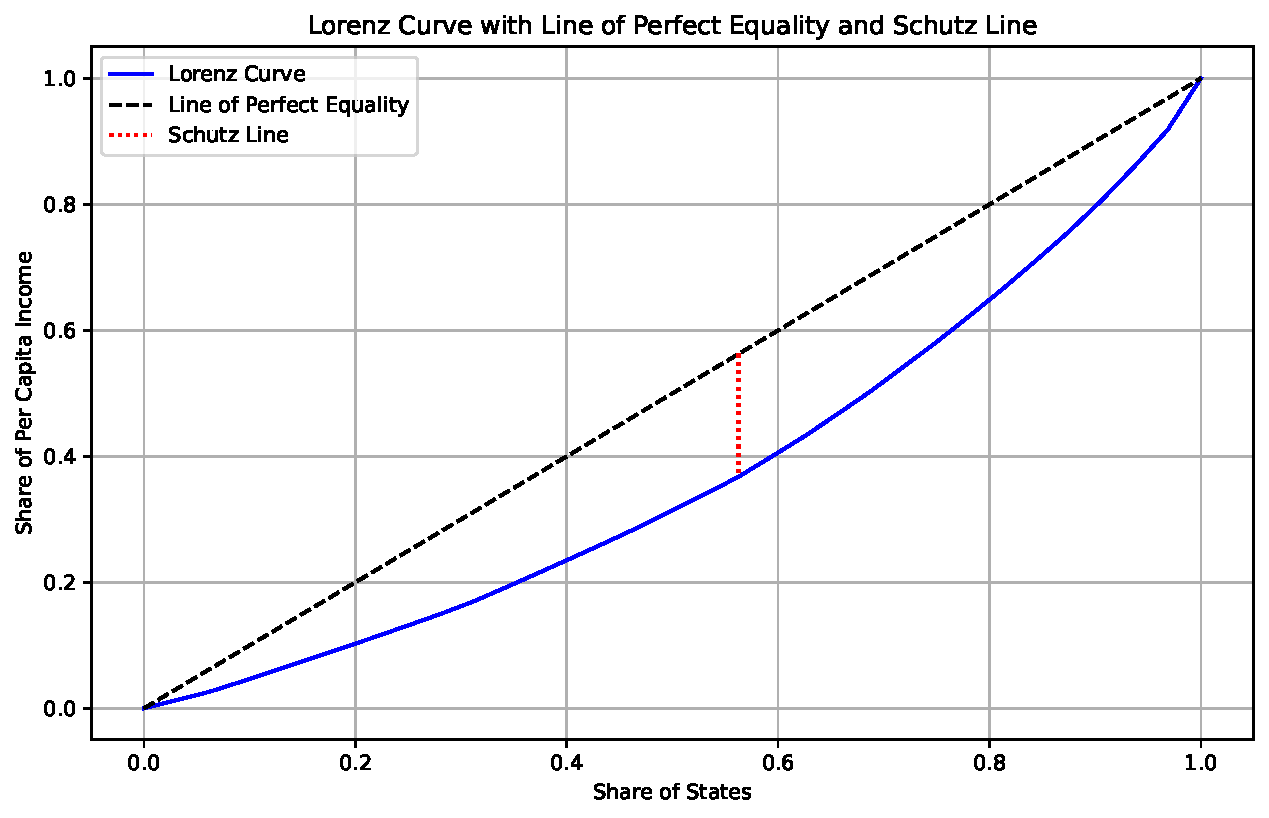
\includegraphics{spatial_inequality_files/figure-pdf/fig-schutz2000-output-1.pdf}

}

\caption{\label{fig-schutz2000}Lorenz Curve and Schutz Line Per Capita
Gross Domestic Product by State 2000}

\end{figure}%

\subsection{Measures of Inequality}\label{measures-of-inequality}

We can derive two indices from the Lorenz curve: the Gini coefficient
and the Schutz coefficient. The Gini coefficient is an area measurement
expressed as a ratio of the area of the lens above the Lorenz curve but
below the diagonal to area under the line of perfect equality. The
Schutz coefficient is a distance measure defined as the maximum vertical
distance between the equality diagonal and the Lorenz curve. Both
coefficients measure the extent to which the Lorenz curve departs from
perfect equality. Moreover, both indices run from 0, perfect equality,
to 1, maximal inequality.

For 2000, the Gini coefficient is 0.258, while the Schutz coefficient is
0.195. As they are both scaled to be within the unit interval, the
temptation is to compare the two values. However, this would be
misleading as we recall one is a measure of area, the second a measure
of distance. Instead, each coefficient is often used to compare across
distributions, either over time or space. We can do this for Mexico by
asking what has happened to inequality over time. Along the way, we add
a third commonly used indicator of inequality, the coefficient of
variation (\(CV\)). The coefficient of variation is a relative measure
of variation as it is defined as the ratio of the standard deviation to
the sample mean.

\begin{Shaded}
\begin{Highlighting}[]
\NormalTok{yvars }\OperatorTok{=}\NormalTok{ [}\SpecialStringTok{f\textquotesingle{}PCGDP}\SpecialCharTok{\{}\NormalTok{year}\SpecialCharTok{\}}\SpecialStringTok{\textquotesingle{}} \ControlFlowTok{for}\NormalTok{ year }\KeywordTok{in}\NormalTok{ years]}
\NormalTok{ginis }\OperatorTok{=}\NormalTok{ [ineq.gini.Gini(gdf[yvar]).g }\ControlFlowTok{for}\NormalTok{ yvar }\KeywordTok{in}\NormalTok{ yvars]}
\NormalTok{res\_df }\OperatorTok{=}\NormalTok{ pd.DataFrame(data}\OperatorTok{=}\NormalTok{ginis, columns}\OperatorTok{=}\NormalTok{[}\StringTok{\textquotesingle{}Gini\textquotesingle{}}\NormalTok{], index}\OperatorTok{=}\NormalTok{years)}
\NormalTok{cv }\OperatorTok{=}\NormalTok{ gdf[yvars].std() }\OperatorTok{/}\NormalTok{ gdf[yvars].mean() }
\NormalTok{res\_df[}\StringTok{\textquotesingle{}CV\textquotesingle{}}\NormalTok{] }\OperatorTok{=}\NormalTok{ cv.values}
\NormalTok{s }\OperatorTok{=}\NormalTok{ [ineq.schutz.Schutz(gdf, yvar).distance }\ControlFlowTok{for}\NormalTok{ yvar }\KeywordTok{in}\NormalTok{ yvars]}
\NormalTok{res\_df[}\StringTok{\textquotesingle{}Schutz\textquotesingle{}}\NormalTok{] }\OperatorTok{=}\NormalTok{ s}
\NormalTok{res\_df[}\StringTok{\textquotesingle{}Gini\_rank\textquotesingle{}}\NormalTok{] }\OperatorTok{=}\NormalTok{ res\_df[}\StringTok{\textquotesingle{}Gini\textquotesingle{}}\NormalTok{].rank()}
\NormalTok{res\_df[}\StringTok{\textquotesingle{}CV\_rank\textquotesingle{}}\NormalTok{] }\OperatorTok{=}\NormalTok{ res\_df[}\StringTok{\textquotesingle{}CV\textquotesingle{}}\NormalTok{].rank()}
\NormalTok{res\_df[}\StringTok{\textquotesingle{}Schutz\_rank\textquotesingle{}}\NormalTok{] }\OperatorTok{=}\NormalTok{ res\_df[}\StringTok{\textquotesingle{}Schutz\textquotesingle{}}\NormalTok{].rank()}
\NormalTok{res\_df}
\end{Highlighting}
\end{Shaded}

\begin{longtable}[]{@{}lllllll@{}}

\caption{\label{tbl-rankings}Inequality Index Rankings}

\tabularnewline

\toprule\noalign{}
& Gini & CV & Schutz & Gini\_rank & CV\_rank & Schutz\_rank \\
\midrule\noalign{}
\endhead
\bottomrule\noalign{}
\endlastfoot
1940 & 0.353724 & 0.719858 & 0.260037 & 7.0 & 7.0 & 7.0 \\
1950 & 0.296446 & 0.624611 & 0.213920 & 6.0 & 6.0 & 6.0 \\
1960 & 0.253718 & 0.492447 & 0.181549 & 3.0 & 3.0 & 3.0 \\
1970 & 0.255134 & 0.472039 & 0.185266 & 4.0 & 2.0 & 4.0 \\
1980 & 0.245053 & 0.462657 & 0.179702 & 1.0 & 1.0 & 1.0 \\
1990 & 0.251818 & 0.497729 & 0.181363 & 2.0 & 5.0 & 2.0 \\
2000 & 0.258113 & 0.492565 & 0.195043 & 5.0 & 4.0 & 5.0 \\

\end{longtable}

Table~\ref{tbl-rankings} shows that the three indices agree that
inequality was lowest in 1980, and the highest in 1940. However, while
the Gini and Schutz coefficients agree in their rankings, the inclusion
of the CV creates discordance. Part of the discordance reflects the
sensitivity of the measures to different parts of the income
distribution. The Gini coefficient puts more weight on the middle of the
distribution, while the CV is more affected by the right tail of the
distribution. The discordance also reflects the property that when the
Lorenz curves do not intersect, the CV and Gini would agree on the
rankings of inequality. However, Figure~\ref{fig-lcs} shows that there
are cases where the Lorenz curves intersect.

The discordance in rankings complicates whether income inequality
between states in Mexico has increased or decreased. The answer now
depends upon which temporal interval one chooses. Both the Gini and CV
agree that inequality has declined since 1940, irrespective of the
terminal year selected. However, they disagree on the answer when the
question is whether inequality decreased from, say, 1960 to 1970 or
between 1990 and 2000 (see Table~\ref{tbl-rankings}).

\begin{Shaded}
\begin{Highlighting}[]
\ImportTok{import}\NormalTok{ pandas }\ImportTok{as}\NormalTok{ pd}
\ImportTok{import}\NormalTok{ numpy }\ImportTok{as}\NormalTok{ np}
\ImportTok{import}\NormalTok{ matplotlib.pyplot }\ImportTok{as}\NormalTok{ plt}
\ImportTok{from}\NormalTok{ scipy.stats }\ImportTok{import}\NormalTok{ cumfreq}

\KeywordTok{def}\NormalTok{ lorenz\_curve(incomes):}
\NormalTok{    sorted\_incomes }\OperatorTok{=}\NormalTok{ np.sort(incomes)}
\NormalTok{    cumulative\_incomes }\OperatorTok{=}\NormalTok{ np.cumsum(sorted\_incomes)}
\NormalTok{    normalized }\OperatorTok{=}\NormalTok{ cumulative\_incomes }\OperatorTok{/}\NormalTok{ cumulative\_incomes[}\OperatorTok{{-}}\DecValTok{1}\NormalTok{]}
\NormalTok{    lorenz\_curve }\OperatorTok{=}\NormalTok{ np.insert(normalized, }\DecValTok{0}\NormalTok{, }\DecValTok{0}\NormalTok{)}
\NormalTok{    n }\OperatorTok{=} \BuiltInTok{len}\NormalTok{(incomes)}
\NormalTok{    x }\OperatorTok{=}\NormalTok{ np.linspace(}\FloatTok{0.0}\NormalTok{, }\FloatTok{1.0}\NormalTok{, n }\OperatorTok{+} \DecValTok{1}\NormalTok{)}
    \ControlFlowTok{return}\NormalTok{ x, lorenz\_curve}


\NormalTok{plt.figure(figsize}\OperatorTok{=}\NormalTok{(}\DecValTok{10}\NormalTok{, }\DecValTok{8}\NormalTok{))}

\ControlFlowTok{for}\NormalTok{ yvar }\KeywordTok{in}\NormalTok{ yvars:}
\NormalTok{    incomes }\OperatorTok{=}\NormalTok{ gdf[yvar].values}
\NormalTok{    x, y }\OperatorTok{=}\NormalTok{ lorenz\_curve(incomes)}
\NormalTok{    plt.plot(x, y, label}\OperatorTok{=}\NormalTok{yvar)}

\CommentTok{\# Plotting the line of equality}
\NormalTok{plt.plot([}\DecValTok{0}\NormalTok{, }\DecValTok{1}\NormalTok{], [}\DecValTok{0}\NormalTok{, }\DecValTok{1}\NormalTok{], color}\OperatorTok{=}\StringTok{\textquotesingle{}black\textquotesingle{}}\NormalTok{, linestyle}\OperatorTok{=}\StringTok{\textquotesingle{}{-}{-}\textquotesingle{}}\NormalTok{)}

\CommentTok{\# Adding titles and labels}
\NormalTok{plt.title(}\StringTok{\textquotesingle{}Lorenz Curves for PCGDP by Year\textquotesingle{}}\NormalTok{)}
\NormalTok{plt.xlabel(}\StringTok{\textquotesingle{}Cumulative Share of States\textquotesingle{}}\NormalTok{)}
\NormalTok{plt.ylabel(}\StringTok{\textquotesingle{}Cumulative Share of PCGDP\textquotesingle{}}\NormalTok{)}
\NormalTok{plt.legend()}
\NormalTok{plt.grid(}\VariableTok{True}\NormalTok{)}
\NormalTok{plt.show()}
\end{Highlighting}
\end{Shaded}

\begin{figure}[H]

\centering{

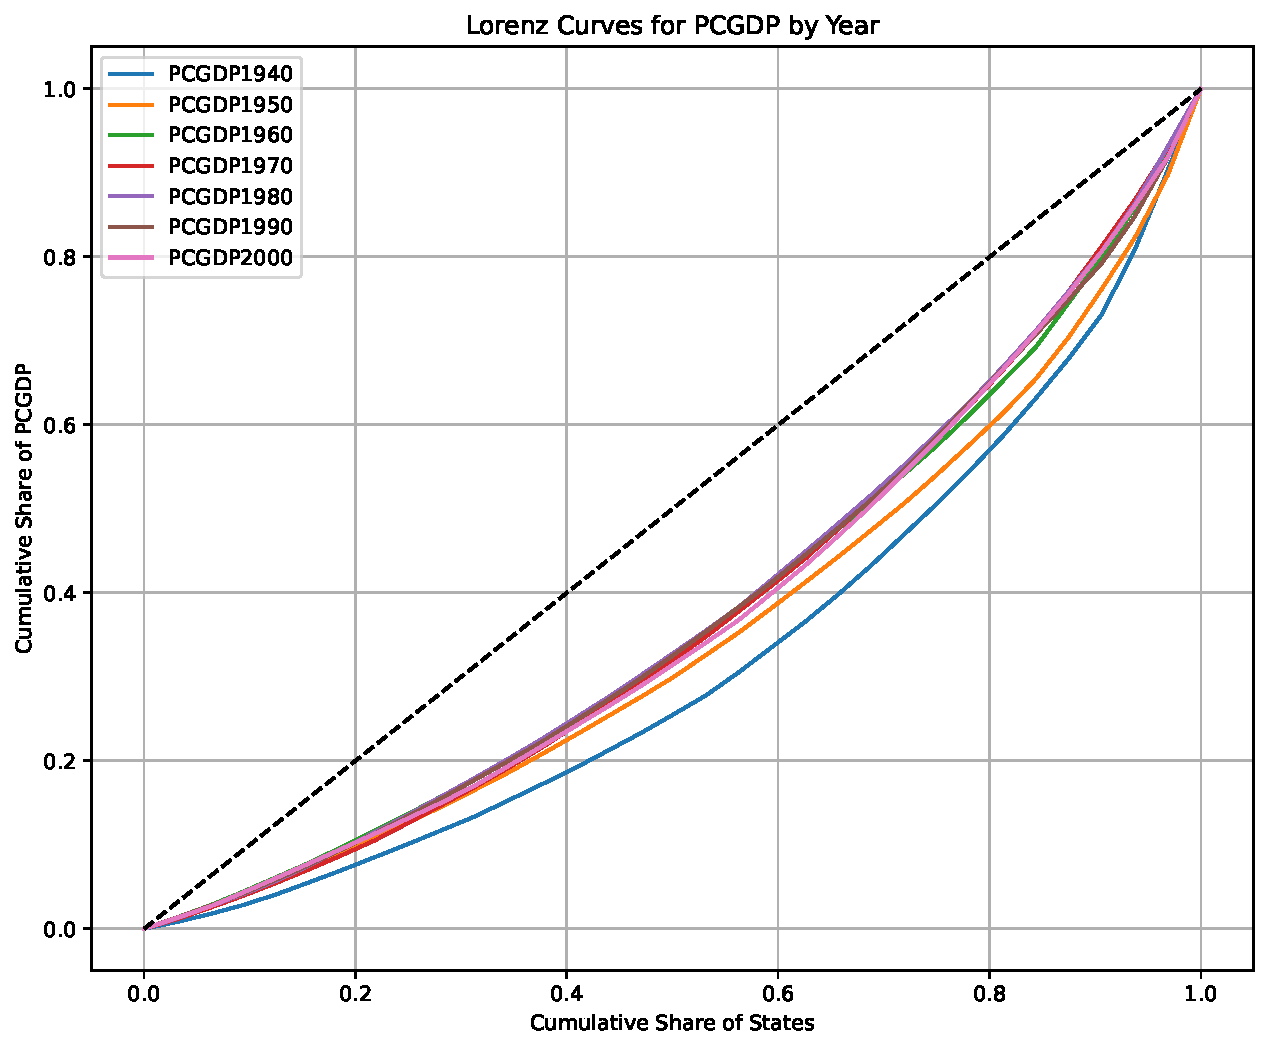
\includegraphics{spatial_inequality_files/figure-pdf/fig-lcs-output-1.pdf}

}

\caption{\label{fig-lcs}Lorenz Curves by Decade}

\end{figure}%

The CV and Gini are but two of a collection of scalar measures of
inequality we could apply. Other commonly employed inequality measures
include the variance, the relative mean deviation, logarithmic variance,
variance of the logarithms, Atkinson, and Theil.\footnote{See
  \citet{cowell2011MeasuringInequality} for an overview of inequality
  measures.} Choosing among the rich diversity of inequality measures
has been the subject of a vast literature. To help guide that selection,
there are five desirable properties of an inequality measure:

\begin{enumerate}
\def\labelenumi{\arabic{enumi}.}
\tightlist
\item
  Symmetry or anonymity
\item
  Principle of transfers
\item
  Scale invariance
\item
  Replication invariance
\item
  Zero normalization
\end{enumerate}

Symmetry implies that the names of the income receiving unit should be
immaterial. That is, if we swap the income of one geographical unit with
that of another, the overall inequality measure should not change. The
principle of transfers implies that the measure should reflect a
reduction in inequality if income is transferred from a richer unit to a
poorer unit, as long as the transfer does not reverse their income
ranking. Scale invariance means that if all incomes are multiplied by
the same constant, inequality remains unchanged. Replication invariance
implies that an inequality measure should be unaffected if the
population is replicated, meaning that duplicating the entire income
distribution does not alter the measure of inequality. Zero
normalization means that an inequality measure assigns a value of zero
to a perfectly equal income distribution, serving as a baseline where
all units have the same income.

Not all of the inequality measures satisfy all of these five properties.
For example, the variance is not scale invariant, and both the
logarithmic variance and variance of logarithms fail the principle of
transfers property. Even for measures that respect these five
properties, their use in comparing the levels of inequality between
countries at one point in time, or the same country at different points
of time, requires the researcher to specify a social welfare function
\citep{atkinson1970MeasurementInequality}.

However, in the study of spatial inequality, it is important to note
that all the measures mentioned above share a sixth property:
\emph{spatial invariance}. This means they are insensitive to the
\emph{geographical} distribution of the income values. The spatial
invariance is demonstrated in Figure~\ref{fig-invariance}, where we
compare two spatial distributions, one that is the actual distribution
for 2000 and one where we artificially permute the incomes randomly.
Despite markedly different spatial patterns, the income distributions
summarized in the histograms in the bottom row are identical. Since all
of the inequality measures mentioned only consider information about the
statistical distribution, each measure will take on the same value
whether applied to the spatial distribution on the left or right of the
figure.

From a geographical perspective, spatial invariance is not a desirable
property in an inequality measure. Let's now turn our attention to
spatially explicit measures of inequality.

\begin{Shaded}
\begin{Highlighting}[]
\NormalTok{fig, axs }\OperatorTok{=}\NormalTok{ plt.subplots(}\DecValTok{2}\NormalTok{, }\DecValTok{2}\NormalTok{)}

\NormalTok{gdf.plot(column}\OperatorTok{=}\StringTok{\textquotesingle{}PCGDP2000\textquotesingle{}}\NormalTok{, ax}\OperatorTok{=}\NormalTok{axs[}\DecValTok{0}\NormalTok{, }\DecValTok{0}\NormalTok{], scheme}\OperatorTok{=}\StringTok{\textquotesingle{}quantiles\textquotesingle{}}\NormalTok{,}
\NormalTok{         cmap}\OperatorTok{=}\StringTok{\textquotesingle{}viridis\textquotesingle{}}\NormalTok{)}
\NormalTok{axs[}\DecValTok{0}\NormalTok{, }\DecValTok{0}\NormalTok{].set\_title(}\StringTok{\textquotesingle{}PCGDP2000\textquotesingle{}}\NormalTok{)}
\NormalTok{axs[}\DecValTok{0}\NormalTok{, }\DecValTok{0}\NormalTok{].axis(}\StringTok{\textquotesingle{}off\textquotesingle{}}\NormalTok{)}


\NormalTok{gdf[}\StringTok{\textquotesingle{}PCGDP2000r\textquotesingle{}}\NormalTok{] }\OperatorTok{=}\NormalTok{ np.random.permutation(gdf.PCGDP2000)}

\NormalTok{gdf.plot(column}\OperatorTok{=}\StringTok{\textquotesingle{}PCGDP2000r\textquotesingle{}}\NormalTok{, ax}\OperatorTok{=}\NormalTok{axs[}\DecValTok{0}\NormalTok{, }\DecValTok{1}\NormalTok{], scheme}\OperatorTok{=}\StringTok{\textquotesingle{}quantiles\textquotesingle{}}\NormalTok{,}
\NormalTok{         cmap}\OperatorTok{=}\StringTok{\textquotesingle{}viridis\textquotesingle{}}\NormalTok{)}
\NormalTok{axs[}\DecValTok{0}\NormalTok{, }\DecValTok{1}\NormalTok{].set\_title(}\StringTok{\textquotesingle{}PCGDP2000 Random\textquotesingle{}}\NormalTok{)}
\NormalTok{axs[}\DecValTok{0}\NormalTok{, }\DecValTok{1}\NormalTok{].axis(}\StringTok{\textquotesingle{}off\textquotesingle{}}\NormalTok{)}

\NormalTok{axs[}\DecValTok{1}\NormalTok{, }\DecValTok{0}\NormalTok{].hist(gdf[}\StringTok{\textquotesingle{}PCGDP2000\textquotesingle{}}\NormalTok{], bins}\OperatorTok{=}\DecValTok{30}\NormalTok{, color}\OperatorTok{=}\StringTok{\textquotesingle{}skyblue\textquotesingle{}}\NormalTok{,}
\NormalTok{               edgecolor}\OperatorTok{=}\StringTok{\textquotesingle{}black\textquotesingle{}}\NormalTok{)}
\NormalTok{axs[}\DecValTok{1}\NormalTok{, }\DecValTok{0}\NormalTok{].set\_title(}\StringTok{\textquotesingle{}PCGDP2000 Histogram\textquotesingle{}}\NormalTok{)}
\NormalTok{axs[}\DecValTok{1}\NormalTok{, }\DecValTok{0}\NormalTok{].set\_xlabel(}\StringTok{\textquotesingle{}PCGDP2000\textquotesingle{}}\NormalTok{)}
\NormalTok{axs[}\DecValTok{1}\NormalTok{, }\DecValTok{0}\NormalTok{].set\_ylabel(}\StringTok{\textquotesingle{}Frequency\textquotesingle{}}\NormalTok{)}

\NormalTok{axs[}\DecValTok{1}\NormalTok{, }\DecValTok{1}\NormalTok{].hist(gdf[}\StringTok{\textquotesingle{}PCGDP2000r\textquotesingle{}}\NormalTok{], bins}\OperatorTok{=}\DecValTok{30}\NormalTok{, color}\OperatorTok{=}\StringTok{\textquotesingle{}skyblue\textquotesingle{}}\NormalTok{,}
\NormalTok{               edgecolor}\OperatorTok{=}\StringTok{\textquotesingle{}black\textquotesingle{}}\NormalTok{)}
\NormalTok{axs[}\DecValTok{1}\NormalTok{, }\DecValTok{1}\NormalTok{].set\_title(}\StringTok{\textquotesingle{}PCGDP2000 Random Histogram\textquotesingle{}}\NormalTok{)}
\NormalTok{axs[}\DecValTok{1}\NormalTok{, }\DecValTok{1}\NormalTok{].set\_xlabel(}\StringTok{\textquotesingle{}PCGDP2000r\textquotesingle{}}\NormalTok{)}
\NormalTok{axs[}\DecValTok{1}\NormalTok{, }\DecValTok{1}\NormalTok{].set\_ylabel(}\StringTok{\textquotesingle{}Frequency\textquotesingle{}}\NormalTok{)}

\NormalTok{plt.tight\_layout()}

\NormalTok{plt.show()}
\end{Highlighting}
\end{Shaded}

\begin{figure}[H]

\centering{

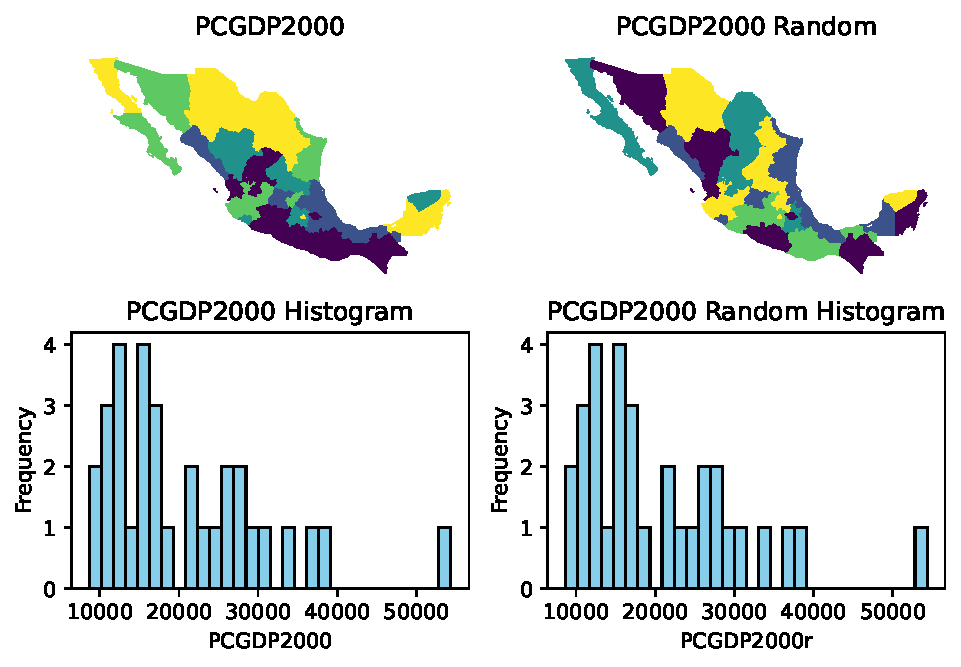
\includegraphics{spatial_inequality_files/figure-pdf/fig-invariance-output-1.pdf}

}

\caption{\label{fig-invariance}Spatial Invariance of Distributions}

\end{figure}%

\subsection{Putting Space into the Measurement of
Inequality}\label{putting-space-into-the-measurement-of-inequality}

The inability of the inequality measures to capture any of the
geographical dimensions of inequality stems from the treatment of the
geographical units of measurement as individuals, and the desire to
respect the principle of symmetry or anonymity that is desired in a
classic inequality measure. This enables researchers to draw upon the
wealth of knowledge about the properties of classic inequality measures,
but at the cost of ignoring geography. In other words, these measures
say a lot about inequality in the statistical distribution of incomes
but they are silent on the spatial distribution of incomes.

In this section, we discuss the approaches used to integrate the spatial
and statistical distributions in the study of spatial inequality. Given
that these methods take the geographical distribution into account, they
can be said to be \emph{spatially explicit measures of inequality}.

These approaches all can be seen as special cases of inequality
decomposition.

\subsubsection{Regional Inequality
Decomposition}\label{regional-inequality-decomposition}

A common approach to introducing geography in the measurement of
inequality leverages the fact that certain inequality measures can be
\emph{decomposed} if the individual income receiving units are placed
into a set of mutually exclusive and exhaustive groups. The
decomposition then identifies the overall inequality that is due to
inequality within groups and between the groups.

To see how this works, we return to the Theil inequality measure that we
mentioned briefly above. Let \(y_i\) be the income of unit \(i\), and
\(s_i\) represent the income share of unit \(i\) such that
\(s_i = \frac{y_i}{\sum_i y_i}\) and \(\sum_i s_i=1\). Then, consider
the distribution of the shares. When all units have the same income
\(s_i = s_j =
1/n\). Then the entropy of the shares given as

\[ H(y) = \sum_{i=1}^n s_i \ln \frac{1}{s_i}\] will be maximized at
\(\ln n\). In the case of extreme inequality, all but one unit have
\(s_i=0\) and a single unit has all income \(s_j=1\), and \(H(y)=0\).
Thus, the entropy function can be viewed as an indicator of \emph{income
equality}.

To generate an indicator of \emph{income inequality}, we can contrast an
observed distribution's equality against the maximum:

\[T(y) = \ln n - H(y) = \ln n - \sum_{i=1}^n s_i \ln \frac{1}{s_i}=\sum_{i=1}^n s_i \ln n s_i.\]

This can be viewed as a weighted average of the logarithmic deviations
of the shares, with the weights defined as the shares. The logarithmic
deviation of share \(i\) from perfect equality is
\(\ln \frac{s_i}{1/n} = \ln s_i n\).

Alternatively, the Theil index can be defined using relative incomes:

\[T = \frac{1}{n} \sum_i \frac{y_i}{\mu} \ln \frac{y_i}{\mu}\] where
\(y_i\) is the income of unit \(i\) and
\(\mu = \frac{1}{n} \sum_i y_i\).

Decomposition of the overall \(T\) measure requires assigning each unit
to exactly one of \(G\) sets \(S_1, S_2, \ldots, S_G\), with the size of
each set given as \(n_g\) so that: \[
\sum_{g=1}^G n_g = n.
\]

Given this, we have:

\[Y_g = \sum_{i \in S_g} y_i \ g=1,\ldots,G\]

Defining \(\omega_g = \frac{n_g}{n} \frac{\bar{Y}_g}{\mu}\), the Theil
index can be rewritten as:

\begin{equation}\phantomsection\label{eq-decomp}{
T = \sum_{g=1}^G \omega_g T_g + \sum_{g=1}^G \omega_g \ln
\frac{\bar{Y}_g}{\mu}.
}\end{equation}

The first term is the within group inequality defined as a weighted
average of the inequality within each group with the weights equal to
the group's share of overall income, with:

\[T_g = \frac{1}{n_g} \sum_{i \in S_g} \frac{y_i}{\bar{Y}_g} \ln \frac{y_i}{\bar{Y}_g}.\]

The second term in Equation~\ref{eq-decomp} is the between group
inequality component, measuring the inequality that would exist if
within each group there was no inequality (i.e., all members of the same
set have the same income).

Decomposition of inequality had been widely applied in economics to
study inequality between occupational groups, sexes, and races, where
individuals would be placed into the mutually exclusive groups and
overall individual inequality decomposed into that due to the
differences between and within the groups. It was a short jump to adopt
this to spatial inequality by using regions to define the groups, with
individual units (in our case, states) being assigned to one and only
one region.\footnote{One of the earliest applications of decomposition
  for regional inequality analysis is
  \citet{theil1967EconomicsInformation}.}

We will illustrate this for the case of Mexican states using a regional
partition due to \citet{hanson1996MexicoIntegration} as shown in
Figure~\ref{fig-components}. This regionalization scheme consists of 5
regions, with the size of the regions ranging from 2 states to 10
states.

\begin{figure}

\centering{

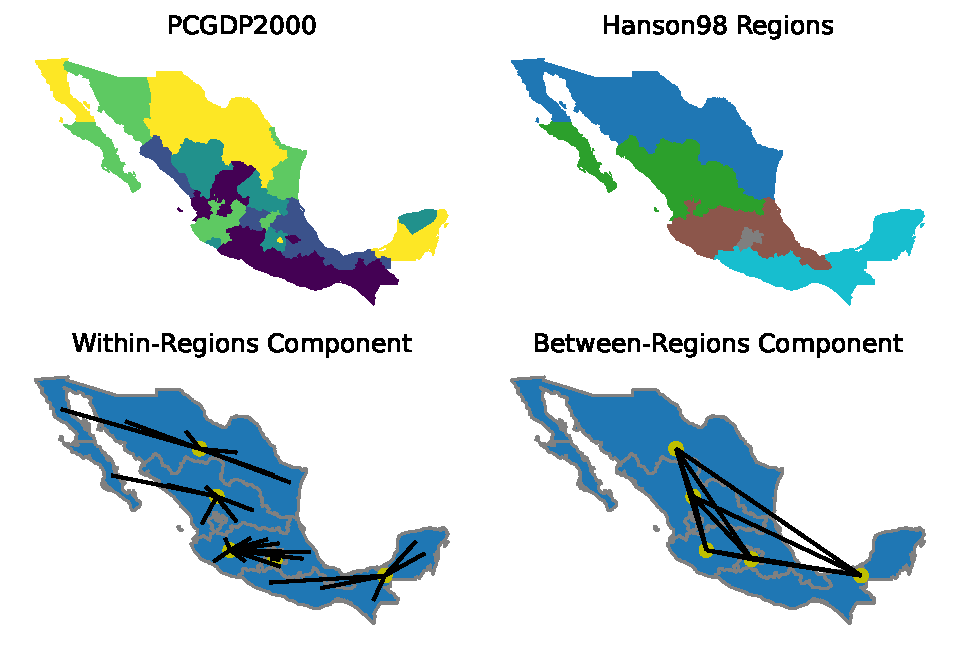
\includegraphics{spatial_inequality_files/figure-pdf/fig-components-output-1.pdf}

}

\caption{\label{fig-components}Regional Inequality Decomposition}

\end{figure}%

We can apply the \texttt{theil} module from \texttt{pysal-inequality} to
calculate the value of the overall level of inequality as measured by
the global Theil index, and its decomposition into the between region
inequality and within region inequality components:

\begin{Shaded}
\begin{Highlighting}[]
\NormalTok{fig, axs }\OperatorTok{=}\NormalTok{ plt.subplots(}\DecValTok{2}\NormalTok{, }\DecValTok{2}\NormalTok{)}
\ImportTok{from}\NormalTok{ inequality.theil }\ImportTok{import}\NormalTok{ TheilDSim}
\NormalTok{np.random.seed(}\DecValTok{12345}\NormalTok{)}

\NormalTok{gdf.plot(}\StringTok{\textquotesingle{}PCGDP2000\textquotesingle{}}\NormalTok{, ax}\OperatorTok{=}\NormalTok{axs[}\DecValTok{0}\NormalTok{, }\DecValTok{0}\NormalTok{], scheme}\OperatorTok{=}\StringTok{\textquotesingle{}quantiles\textquotesingle{}}\NormalTok{,}
\NormalTok{         cmap}\OperatorTok{=}\StringTok{\textquotesingle{}viridis\textquotesingle{}}\NormalTok{)}
\NormalTok{axs[}\DecValTok{0}\NormalTok{, }\DecValTok{0}\NormalTok{].set\_title(}\StringTok{\textquotesingle{}PCGDP2000\textquotesingle{}}\NormalTok{)}
\NormalTok{axs[}\DecValTok{0}\NormalTok{, }\DecValTok{0}\NormalTok{].axis(}\StringTok{\textquotesingle{}off\textquotesingle{}}\NormalTok{)}

\CommentTok{\# Extract the per capita GDP and regimes}
\NormalTok{income }\OperatorTok{=}\NormalTok{ gdf[}\StringTok{\textquotesingle{}PCGDP2000\textquotesingle{}}\NormalTok{]}
\NormalTok{regimes }\OperatorTok{=}\NormalTok{ gdf[}\StringTok{\textquotesingle{}HANSON98\textquotesingle{}}\NormalTok{]}

\NormalTok{res }\OperatorTok{=}\NormalTok{ TheilDSim(income, regimes, }\DecValTok{999}\NormalTok{)}

\NormalTok{gdf[}\StringTok{\textquotesingle{}PCGDP2000r\textquotesingle{}}\NormalTok{] }\OperatorTok{=}\NormalTok{ np.random.permutation(gdf.PCGDP2000)}
\NormalTok{gdf.plot(column}\OperatorTok{=}\StringTok{\textquotesingle{}PCGDP2000r\textquotesingle{}}\NormalTok{, ax}\OperatorTok{=}\NormalTok{axs[}\DecValTok{0}\NormalTok{, }\DecValTok{1}\NormalTok{], scheme}\OperatorTok{=}\StringTok{\textquotesingle{}quantiles\textquotesingle{}}\NormalTok{,}
\NormalTok{         cmap}\OperatorTok{=}\StringTok{\textquotesingle{}viridis\textquotesingle{}}\NormalTok{)}
\NormalTok{axs[}\DecValTok{0}\NormalTok{, }\DecValTok{1}\NormalTok{].set\_title(}\StringTok{\textquotesingle{}PCGDP2000 Random\textquotesingle{}}\NormalTok{)}
\NormalTok{axs[}\DecValTok{0}\NormalTok{, }\DecValTok{1}\NormalTok{].axis(}\StringTok{\textquotesingle{}off\textquotesingle{}}\NormalTok{)}



\NormalTok{gdf[}\StringTok{\textquotesingle{}PCGDP2000r\textquotesingle{}}\NormalTok{] }\OperatorTok{=}\NormalTok{ np.random.permutation(gdf.PCGDP2000)}
\NormalTok{gdf.plot(column}\OperatorTok{=}\StringTok{\textquotesingle{}PCGDP2000r\textquotesingle{}}\NormalTok{, ax}\OperatorTok{=}\NormalTok{axs[}\DecValTok{1}\NormalTok{, }\DecValTok{0}\NormalTok{], scheme}\OperatorTok{=}\StringTok{\textquotesingle{}quantiles\textquotesingle{}}\NormalTok{,}
\NormalTok{         cmap}\OperatorTok{=}\StringTok{\textquotesingle{}viridis\textquotesingle{}}\NormalTok{)}
\NormalTok{axs[}\DecValTok{1}\NormalTok{, }\DecValTok{0}\NormalTok{].set\_title(}\StringTok{\textquotesingle{}PCGDP2000 Random\textquotesingle{}}\NormalTok{)}
\NormalTok{axs[}\DecValTok{1}\NormalTok{, }\DecValTok{0}\NormalTok{].axis(}\StringTok{\textquotesingle{}off\textquotesingle{}}\NormalTok{)}

\NormalTok{msg}\OperatorTok{=}\SpecialStringTok{f\textquotesingle{}Spatial polarization: }\SpecialCharTok{\{}\NormalTok{res}\SpecialCharTok{.}\NormalTok{bg[}\DecValTok{0}\NormalTok{][}\DecValTok{0}\NormalTok{]}\OperatorTok{/}\NormalTok{res}\SpecialCharTok{.}\NormalTok{T}\SpecialCharTok{:.3f\}}\SpecialStringTok{\textquotesingle{}}
\NormalTok{msg}\OperatorTok{=}\SpecialStringTok{f\textquotesingle{}}\SpecialCharTok{\{}\NormalTok{msg}\SpecialCharTok{\}}\SpecialStringTok{, pseudo p{-}value: }\SpecialCharTok{\{}\NormalTok{res}\SpecialCharTok{.}\NormalTok{bg\_pvalue[}\DecValTok{0}\NormalTok{]}\SpecialCharTok{\}}\SpecialStringTok{\textquotesingle{}}
\BuiltInTok{print}\NormalTok{(msg)}
\NormalTok{realizations }\OperatorTok{=}\NormalTok{ np.array([t.bg}\OperatorTok{/}\NormalTok{t.T }\ControlFlowTok{for}\NormalTok{ t }\KeywordTok{in}\NormalTok{ res.results])}
\BuiltInTok{print}\NormalTok{(}\SpecialStringTok{f\textquotesingle{}Ho mean: }\SpecialCharTok{\{}\NormalTok{realizations}\SpecialCharTok{.}\NormalTok{mean()}\SpecialCharTok{:.3f\}}\SpecialStringTok{\textquotesingle{}}\NormalTok{)}

\NormalTok{kde }\OperatorTok{=}\NormalTok{ sns.kdeplot(realizations, fill}\OperatorTok{=}\VariableTok{False}\NormalTok{, color}\OperatorTok{=}\StringTok{\textquotesingle{}blue\textquotesingle{}}\NormalTok{, ax}\OperatorTok{=}\NormalTok{axs[}\DecValTok{1}\NormalTok{,}\DecValTok{1}\NormalTok{])}
\NormalTok{x, y }\OperatorTok{=}\NormalTok{ kde.get\_lines()[}\DecValTok{0}\NormalTok{].get\_data()}
\NormalTok{plt.legend([], [], frameon}\OperatorTok{=}\VariableTok{False}\NormalTok{)}
\CommentTok{\# Fill the area to the right of the specified value}
\NormalTok{plt.fill\_between(x, y, where}\OperatorTok{=}\NormalTok{(x }\OperatorTok{\textgreater{}=}\NormalTok{ realizations[}\DecValTok{0}\NormalTok{]),}
\NormalTok{                 interpolate}\OperatorTok{=}\VariableTok{True}\NormalTok{, color}\OperatorTok{=}\StringTok{\textquotesingle{}red\textquotesingle{}}\NormalTok{, alpha}\OperatorTok{=}\FloatTok{0.5}\NormalTok{)}

\CommentTok{\# Add vertical line at the specified value}
\NormalTok{plt.axvline(x}\OperatorTok{=}\NormalTok{realizations[}\DecValTok{0}\NormalTok{], color}\OperatorTok{=}\StringTok{\textquotesingle{}red\textquotesingle{}}\NormalTok{, linestyle}\OperatorTok{=}\StringTok{\textquotesingle{}{-}{-}\textquotesingle{}}\NormalTok{)}
\NormalTok{plt.xlabel(}\StringTok{"Spatial Polarization"}\NormalTok{)}
\BuiltInTok{print}\NormalTok{(}\SpecialStringTok{f\textquotesingle{}Theil: }\SpecialCharTok{\{}\NormalTok{res}\SpecialCharTok{.}\NormalTok{T}\SpecialCharTok{\}}\SpecialStringTok{\textquotesingle{}}\NormalTok{)}
\BuiltInTok{print}\NormalTok{(}\SpecialStringTok{f\textquotesingle{}KB p{-}value: }\SpecialCharTok{\{}\NormalTok{(realizations }\OperatorTok{\textgreater{}=}\NormalTok{ realizations[}\DecValTok{0}\NormalTok{])}\SpecialCharTok{.}\BuiltInTok{sum}\NormalTok{()}\OperatorTok{/}\DecValTok{1000}\SpecialCharTok{\}}\SpecialStringTok{\textquotesingle{}}\NormalTok{)}
\end{Highlighting}
\end{Shaded}

\begin{verbatim}
Spatial polarization: 0.341, pseudo p-value: 0.036
Ho mean: 0.139
Theil: 0.10660832349588023
KB p-value: 0.036
\end{verbatim}

\begin{figure}[H]

\centering{

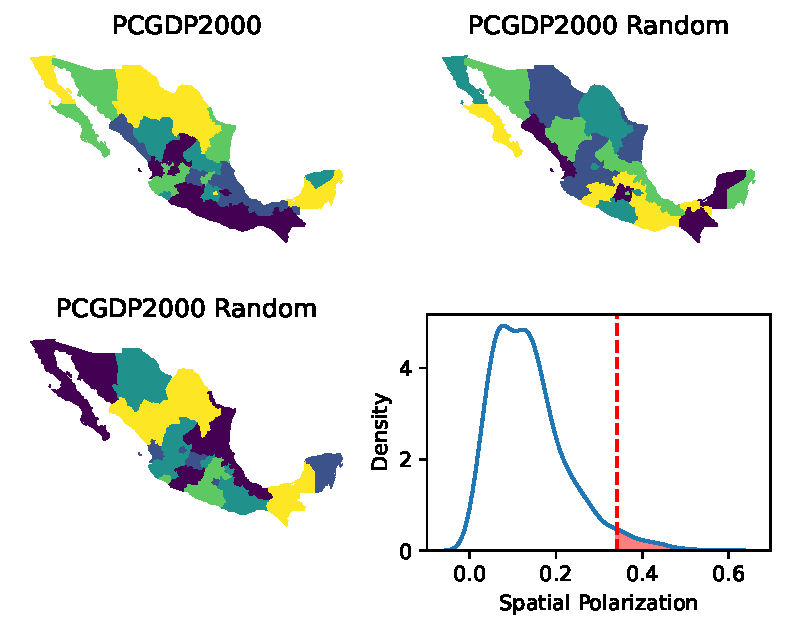
\includegraphics{spatial_inequality_files/figure-pdf/fig-polarization-output-2.pdf}

}

\caption{\label{fig-polarization}Spatial Polarization}

\end{figure}%

The overall level of regional inequality is 0.106. The between region
component stands at 0.036, while the within region element is 0.070. In
relative terms, inequality between the regions in Mexico accounts for 34
percent of state income inequality, while inequality between states from
the same region is the larger share presenting 72 percent of spatial
inequality.

The ratio of between to within region inequality has been suggested as a
measure of \emph{spatial polarization} \citep{zhang2001WhatDifference}.
Since the two components sum to overall inequality, we can re-express
the measure of spatial polarization as the ratio of between region to
overall inequality. Thus, the level of spatial polarization of state
incomes stood at 34 percent in 2000 in Mexico.

A relevant question here is whether this level of spatial polarization
in 2000 should be considered high or not? Another way to express this,
is to ask if the polarization is higher than we would expect if state
incomes were randomly distributed in space in Mexico in 2000.

We can answer this question by developing counter-factual spatial
distributions that reflect a null hypothesis of spatially random income
distributions. Given the \(n\) observations, in our case states, there
are \(n!\) permutations of incomes that are equally likely. In
Figure~\ref{fig-polarization}, the maps in the top-right and lower-left
are two such realizations, where the observed incomes from 2000
(top-left) have been randomly reassigned to states.

Since it is not feasible to generate all \(32!\) maps in our
case,\footnote{\(32! = 2.6313084e+35\).} we take a sample of 999 such
maps from the distribution of permutations. For each of these maps we
calculate the spatial polarization measure, and collect all measures to
develop a reference distribution for our index under the null of
spatially random income distributions. We evaluate our observed spatial
polarization index against this distribution and derive a pseudo p-value
as the number of counterfactual distributions that generate polarization
levels as large as the observed value over the number of permutations
plus one.

The reference distribution for the polarization index is reported in the
bottom right of Figure~\ref{fig-polarization}. The area to the right of
our observed polarization index of 0.34 is 0.036 of the distribution. By
convention, this p-value points to a significant departure from the
null, and we would conclude that the level of spatial polarization of
incomes in Mexico is significantly different from that expected were
incomes generated by a spatially random process.

The regional decomposition is a spatially explicit measure of spatial
inequality as it is indeed sensitive to the geographical distribution of
the income values. It is important to note, however, that it is the
spatial polarization index, and not the overall \(T\) that is spatially
explicit. Each of the counterfactual spatial distributions used to
construct the reference distribution for the spatial polarization index
would still have the same attribute distribution, with similar means and
variances, and levels of overall inequality.

While the regional inequality decomposition is spatially explicit, it
treats geography in an aggregated fashion. There are, in essence, two
scales of spatial inequality implied in this decomposition. As displayed
in Figure~\ref{fig-components}, the within-regions component might be
considered the ``local'' measure as it compares incomes belonging to the
same region to the mean income of the group. The between-regions
inequality component, by contrast, views spatial inequality in a more
aggregate fashion considering only the differences in regional means.

A close inspection of the decomposition Equation~\ref{eq-decomp} reveals
both the within and between inequality components are functions of a
\(T\) index. In the former case this is applied to states from the same
region, and in the latter case, the \(T\) is applied to the means of
regional incomes. For the within region component, the actual spatial
distribution of the member states within each of their regions is
ignored. By the same token, the geographical location of the regions is
immaterial to the calculation of the between region component. In other
words, once the states have been assigned to regions, geography no
longer matters. Thus, we draw a distinction between \emph{regional}
inequality decomposition and \emph{spatial} inequality decomposition.

\subsubsection{Spatial Inequality
Decomposition}\label{spatial-inequality-decomposition}

To capture these ignored dimensions of the spatial distribution,
\citet{rey2013SpatialDecomposition} suggested a spatial decomposition of
the Gini coefficient. Starting from the Gini coefficient expressed as
half the relative mean absolute deviation:\footnote{It is sometimes
  stated that the maximum value of the Gini in this form is 1
  \citep[e.g.,][]{wang2024RobustMethod}. This is technically incorrect,
  as in in this form, the Gini has a range of \([0, (n-1)/n]\). As \(n\)
  grows larger, the upper bound approaches 1. Moreover, because the
  upper bound is a function of \(n\), care should be taken when using
  the Gini in this form when comparing distributions of different sizes.}
\begin{equation}\phantomsection\label{eq-gini-mad}{
Gini = \sum_{i=1}^n \sum_{j=1}^n \frac{|y_i - y_j|}{2n^2 \bar{y}}
}\end{equation} the sum of the absolute deviations can be decomposed as:
\begin{equation}\phantomsection\label{eq-gini-sad}{
\sum_{i=1}^n \sum_{j=1}^n |y_i - y_j| = \sum_{i=1}^n \sum_{j=1}^n w_{i,j} |y_i -
y_j| + (1-w_{i,j})\sum_{i=1}^n \sum_{j=1}^n |y_i - y_j|
}\end{equation} where \(w_{i,j} = 1\) if states \(i\) and \(j\) are
geographical neighbors, \(w_{i,j}=0\) otherwise. Here we define
neighbors as states that share a border.

Substituting Equation~\ref{eq-gini-sad} into Equation~\ref{eq-gini-mad}
gives: \begin{equation}\phantomsection\label{eq-gini-spatial}{
Gini = \sum_{i=1}^n \sum_{j=1}^n \frac{w_{i,j} |y_i - y_j|}{2n^2 \bar{y}} +
\sum_{i=1}^n \sum_{j=1}^n \frac{ (1-w_{i,j}) |y_i - y_j|}{2n^2 \bar{y}}
}\end{equation} The first term represents a measure of inequality
between neighboring states, while the second term captures inequality
between ``distant'' pairs of states. For most spatial configurations,
the number of neighboring pairs will be dwarfed by the number of pairs
of states that are distant. So while, in the case of spatially clustered
income values, the expectation would be for the average difference in
incomes to be smaller for neighboring rather than distant states, our
measure of spatial clustering here has to take into account the
different cardinality of the two sets of pairs. As such, the relevant
comparison is if the first term (second term) is smaller (larger) than
what could be expected if state incomes were randomly distributed in
space.

We apply the Spatial Gini Decomposition to Mexican State incomes in 2000
using \texttt{pysal-inequality} in Figure~\ref{fig-gini-spatial}. The
adjacency graph based on the criterion of Queen neighbors is shown in
the top-right figure. An edge defines a pair of neighboring states.

\begin{Shaded}
\begin{Highlighting}[]
\NormalTok{fig, axs }\OperatorTok{=}\NormalTok{ plt.subplots(}\DecValTok{2}\NormalTok{, }\DecValTok{2}\NormalTok{)}
\ImportTok{from}\NormalTok{ inequality.gini }\ImportTok{import}\NormalTok{ Gini\_Spatial}
\ImportTok{import}\NormalTok{ libpysal}
\NormalTok{np.random.seed(}\DecValTok{12345}\NormalTok{)}


\NormalTok{gdf.plot(}\StringTok{\textquotesingle{}PCGDP2000\textquotesingle{}}\NormalTok{, ax}\OperatorTok{=}\NormalTok{axs[}\DecValTok{0}\NormalTok{, }\DecValTok{0}\NormalTok{], scheme}\OperatorTok{=}\StringTok{\textquotesingle{}quantiles\textquotesingle{}}\NormalTok{, cmap}\OperatorTok{=}\StringTok{\textquotesingle{}viridis\textquotesingle{}}\NormalTok{)}
\NormalTok{axs[}\DecValTok{0}\NormalTok{, }\DecValTok{0}\NormalTok{].set\_title(}\StringTok{\textquotesingle{}PCGDP2000\textquotesingle{}}\NormalTok{)}
\NormalTok{axs[}\DecValTok{0}\NormalTok{, }\DecValTok{0}\NormalTok{].axis(}\StringTok{\textquotesingle{}off\textquotesingle{}}\NormalTok{)}


\NormalTok{wq }\OperatorTok{=}\NormalTok{ libpysal.weights.Queen.from\_dataframe(gdf)}
\NormalTok{wq.transform }\OperatorTok{=} \StringTok{\textquotesingle{}B\textquotesingle{}}
\NormalTok{gs2000 }\OperatorTok{=}\NormalTok{ Gini\_Spatial(gdf[}\StringTok{"PCGDP2000"}\NormalTok{], wq)}

\NormalTok{income }\OperatorTok{=}\NormalTok{ gdf[}\StringTok{\textquotesingle{}PCGDP1940\textquotesingle{}}\NormalTok{]}

\NormalTok{gdf.plot(ax}\OperatorTok{=}\NormalTok{axs[}\DecValTok{0}\NormalTok{, }\DecValTok{1}\NormalTok{])}
\NormalTok{axs[}\DecValTok{0}\NormalTok{, }\DecValTok{1}\NormalTok{].set\_title(}\StringTok{\textquotesingle{}Neighbor Graph\textquotesingle{}}\NormalTok{)}
\NormalTok{axs[}\DecValTok{0}\NormalTok{, }\DecValTok{1}\NormalTok{].axis(}\StringTok{\textquotesingle{}off\textquotesingle{}}\NormalTok{)}


\NormalTok{wq.plot(gdf, ax}\OperatorTok{=}\NormalTok{axs[}\DecValTok{0}\NormalTok{,}\DecValTok{1}\NormalTok{])}

\NormalTok{axs[}\DecValTok{1}\NormalTok{, }\DecValTok{0}\NormalTok{].set\_title(}\StringTok{\textquotesingle{}Counterfactual\textquotesingle{}}\NormalTok{)}
\NormalTok{axs[}\DecValTok{1}\NormalTok{, }\DecValTok{0}\NormalTok{].axis(}\StringTok{\textquotesingle{}off\textquotesingle{}}\NormalTok{)}
\NormalTok{gdf[}\StringTok{\textquotesingle{}PCGDP2000r\textquotesingle{}}\NormalTok{] }\OperatorTok{=}\NormalTok{ np.random.permutation(gdf.PCGDP2000)}
\NormalTok{gdf.plot(column}\OperatorTok{=}\StringTok{\textquotesingle{}PCGDP2000r\textquotesingle{}}\NormalTok{, ax}\OperatorTok{=}\NormalTok{axs[}\DecValTok{1}\NormalTok{,}\DecValTok{0}\NormalTok{], scheme}\OperatorTok{=}\StringTok{\textquotesingle{}quantiles\textquotesingle{}}\NormalTok{,}
\NormalTok{         cmap}\OperatorTok{=}\StringTok{\textquotesingle{}viridis\textquotesingle{}}\NormalTok{)}

\NormalTok{adsum }\OperatorTok{=}\NormalTok{ gs2000.dtotal}
\NormalTok{realizations }\OperatorTok{=}\NormalTok{ gs2000.wcgp }\OperatorTok{/}\NormalTok{ adsum}
\NormalTok{kde }\OperatorTok{=}\NormalTok{ sns.kdeplot(realizations, fill}\OperatorTok{=}\VariableTok{False}\NormalTok{, color}\OperatorTok{=}\StringTok{\textquotesingle{}blue\textquotesingle{}}\NormalTok{, ax}\OperatorTok{=}\NormalTok{axs[}\DecValTok{1}\NormalTok{,}\DecValTok{1}\NormalTok{])}
\NormalTok{x, y }\OperatorTok{=}\NormalTok{ kde.get\_lines()[}\DecValTok{0}\NormalTok{].get\_data()}
\NormalTok{plt.legend([], [], frameon}\OperatorTok{=}\VariableTok{False}\NormalTok{)}
\CommentTok{\# Fill the area to the right of the specified value}
\NormalTok{plt.fill\_between(x, y, where}\OperatorTok{=}\NormalTok{(x }\OperatorTok{\textgreater{}=}\NormalTok{ gs2000.wcg}\OperatorTok{/}\NormalTok{adsum),}
\NormalTok{                 interpolate}\OperatorTok{=}\VariableTok{True}\NormalTok{, color}\OperatorTok{=}\StringTok{\textquotesingle{}red\textquotesingle{}}\NormalTok{, alpha}\OperatorTok{=}\FloatTok{0.5}\NormalTok{)}

\CommentTok{\# Add vertical line at the specified value}
\NormalTok{plt.axvline(x}\OperatorTok{=}\NormalTok{gs2000.wcg}\OperatorTok{/}\NormalTok{adsum, color}\OperatorTok{=}\StringTok{\textquotesingle{}red\textquotesingle{}}\NormalTok{, linestyle}\OperatorTok{=}\StringTok{\textquotesingle{}{-}{-}\textquotesingle{}}\NormalTok{)}
\NormalTok{plt.xlabel(}\StringTok{"Spatial Gini"}\NormalTok{)}


\NormalTok{plt.tight\_layout()}
\NormalTok{plt.show()}
\NormalTok{G }\OperatorTok{=}\NormalTok{ gs2000}
\NormalTok{msg }\OperatorTok{=} \SpecialStringTok{f\textquotesingle{}Expected Distant SADS/Total SADS: }\SpecialCharTok{\{}\NormalTok{G}\SpecialCharTok{.}\NormalTok{e\_wcg}\OperatorTok{/}\NormalTok{adsum}\SpecialCharTok{:.2f\}}\SpecialStringTok{\textquotesingle{}}
\NormalTok{msg }\OperatorTok{=} \SpecialStringTok{f\textquotesingle{}}\SpecialCharTok{\{}\NormalTok{msg}\SpecialCharTok{\}}\SpecialStringTok{, Observed: }\SpecialCharTok{\{}\NormalTok{G}\SpecialCharTok{.}\NormalTok{wcg}\OperatorTok{/}\NormalTok{adsum}\SpecialCharTok{:.2f\}}\CharTok{\textbackslash{}n}\SpecialStringTok{ p{-}value: }\SpecialCharTok{\{}\NormalTok{G}\SpecialCharTok{.}\NormalTok{p\_sim}\SpecialCharTok{\}}\SpecialStringTok{\textquotesingle{}}
\BuiltInTok{print}\NormalTok{(msg)}
\end{Highlighting}
\end{Shaded}

\begin{figure}[H]

\centering{

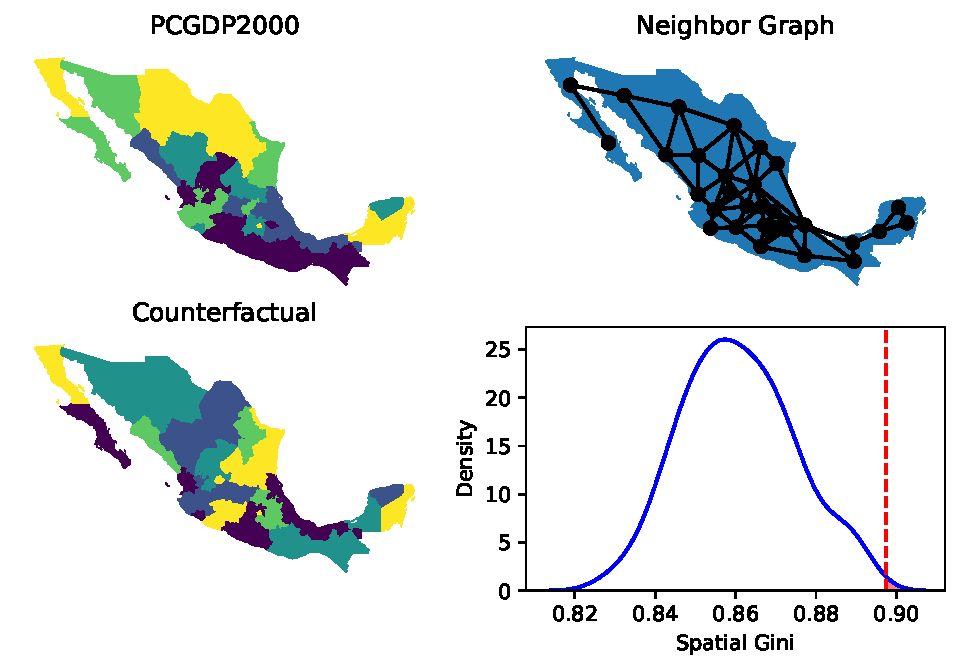
\includegraphics{spatial_inequality_files/figure-pdf/fig-gini-spatial-output-1.pdf}

}

\caption{\label{fig-gini-spatial}Spatial Inequality Decomposition}

\end{figure}%

\begin{verbatim}
Expected Distant SADS/Total SADS: 0.86, Observed: 0.90
 p-value: 0.01
\end{verbatim}

For inference on the spatial Gini, the same computationally based
approach that we used in the Theil decomposition is employed. One of the
counterfactuals representing a random permutation of the incomes is
shown in the lower-left figure. The reference distribution for the
spatial Gini index is shown on the bottom right. Here the spatial Gini
is expressed as the share of the overall absolute pair-wise differences
due to inequality between distant (non-neighbor) pairs of states. The
pseudo p-value (0.01) for the observed index is calculated as the area
to its right under the distribution.

Under the null, the distant pairs should account for 86 percent of the
absolute differences, however, the observed share is much higher at 90
percent. In fact, the p-value indicates that none of the counterfactual
spatial distributions of income generated a spatial Gini as large as the
one observed. In other words, the inequality between distant pairs of
states is larger than the inequality between neighboring states. This
pairwise orientation of the spatial Gini decomposition offers a useful
complement over the regional decomposition of the Theil approach, as it
introduces a more spatially explicit view of the income distribution
that demonstrates how spatial autocorrelation affects overall inequality
across the states.\footnote{For a recent extension of the spatial Gini
  decomposition see \citet{panzera2020MeasuringSpatial}.}

It should be noted that the spatial Gini decomposition does not allow
for the exact additivity of within-group and between-group inequality
components. This is because the Gini index is affected by the degree of
overlap in incomes of states belonging to different regions. Any overlap
complicates the decomposition because part of the total inequality
arises from the overlap itself, which cannot be easily attributed to
either within-group or between-group inequality. So instead of a two-way
additive decomposition, a residual term is required due to the overlap.
Because this residual term is difficult to interpret, the Gini is seldom
used for regional inequality decomposition.

\subsubsection{Weighted or Unweighted Inequality: Places versus
People}\label{weighted-or-unweighted-inequality-places-versus-people}

A final issue we explore is the question of whether the measure of
spatial inequality should take into account the population sizes of the
enumeration units. This was briefly mentioned earlier in the context of
measuring international inequality. In the regional literature, a debate
rages as to whether population weighted or unweighted approaches should
be used to measure spatial inequality
\citep{gluschenko2018MeasuringRegional} .

To frame the debate, it is helpful to consider three different concepts
of inequality at the international scale suggested by
\citet{milanovic2007WorldsApart}. Here we adapt them to the question of
measuring spatial inequality at the sub-national scale. Concept 1 is
unweighted spatial inequality, where each state is one unit of
measurement, and we use its per capita income irrespective of the
state's population. In addition to being the dominant approach in
regional inequality analysis, this concept is at the core of the
literature on regional convergence \citep{rey1999us} where the focus is
on whether the incomes of poor and rich states in a system are coming
together or growing apart over time.

Concept 2 takes into account the population of the individual states,
recognizing that a state like Nuevo Leon with a population of 8.6
million in 2000 having its average income increase by 10,000 USD is
likely to have a larger impact than is seeing the per capita income of
Colima, with a population of 500,000 change by the same amount. So here,
the per capita incomes of the states are now weighted by the population
of the states. This is weighted spatial inequality.

Finally, Concept 3, measures inequality between all the individuals in
the country. Here we would require information on the individuals both
in terms of their incomes and their state of residence. Were it
available, such data would allow us to measure personal income
inequality. However, in the literature on regional inequality, such data
is scarce, and so this concept is not operationalized.

This means the debate in the regional literature is between proponents
of Concept 1 and Concept 2.

Thus far in this paper, we have adopted the Concept 1 definition of
spatial inequality, that is, unweighted spatial inequality. We can
contrast this with the perspective offered by Concept 2, by developing
the Weighted Pengram under concept 2 shown in
Figure~\ref{fig-weighted-pengram} and comparing it with the Unweighted
Pengram from Figure~\ref{fig-pen2000}. The number of bars for each state
in the Weighted Pengram is proportional to the population of that state.
The logic behind the weighted spatial inequality is that rather than
having one representative observation (individual) from the state with
their level of income equal to the state per capita income, now there
are a proportional number of individuals from each state having their
level of income equal to the state's per capita income.

\begin{figure}

\centering{

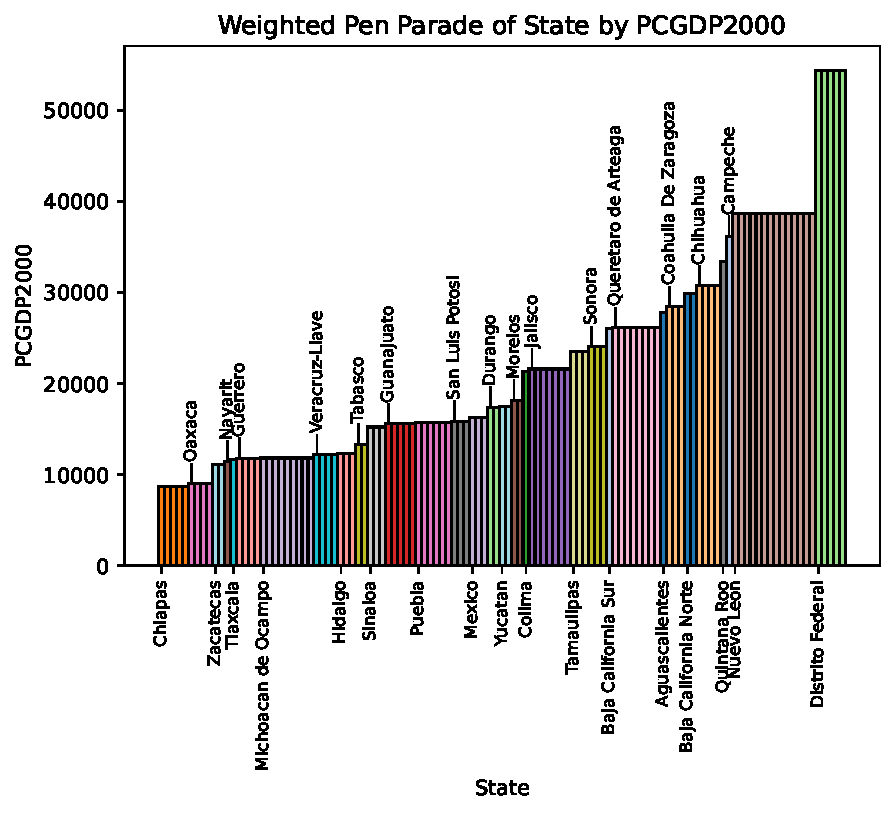
\includegraphics{spatial_inequality_files/figure-pdf/fig-weighted-pengram-output-1.pdf}

}

\caption{\label{fig-weighted-pengram}Populated Weighted Pengram}

\end{figure}%

A fundamental issue with this approach is that it assumes that
inequality among individuals within the state is zero, since all members
have the same level of income. This also implies that for two states
that have different levels of per capita income, the poorest members of
the richer state will be richer than the richest member of the poorer
state. This is at odds with empirical reality.

\section{Conclusion}\label{conclusion}

Regional inequality continues to attract the attention of researchers
and policy makers alike. This chapter has presented the key
methodological approaches available to researchers interested in
analyzing spatial disparities. By highlighting the challenges posed in
adapting classical inequality measures to the question of spatial
inequality, the chapter draws important distinctions between different
types of inequality decomposition approaches based on their treatment of
space. These methods reveal the spatial dimensions of inequality,
particularly the extent to which income disparities are geographically
clustered.

While the focus has been on regional inequality at the sub-national
scale, these methods have a broad scope that researchers can apply at
different spatial scales, from analyzing geographical disparities at the
international level \citep{redding2004EconomicGeography}, inter-regional
\citep{bathelt2024NatureCauses}, as well as intra-urban scale
\citep{oecd2018DividedCities}. This scope is vital, as the mechanisms of
inequality can differ at each scale. For example, trade policy likely
plays a more significant role on an international scale. At the same
time, industrial restructuring is more influential on an inter-regional
scale, and residential sorting is operative on an intra-urban scale.
Furthermore, the resulting patterns of spatial inequality may also vary
across these scales. The work by \citet{ganong2017WhyHas} shows a
substantial divergence of incomes across states but reports a more mixed
pattern when measuring convergence using labor market areas.

Linking the spatial inequality measures to possible policy interventions
offers some possibilities. For example, the distinction between
inter-regional (between-region) and intra-regional (within-region)
inequality in the decomposition may help researchers and policymakers
design such interventions in a tailored fashion. If between-region
inequality dominates, there may be a strong case for place-based
policies. Conversely, if the within-region inequality component accounts
for the majority share, more nationally oriented policies, such as
federal tax laws, may be more appropriate.

In future research, it would be beneficial to investigate the
relationship between spatial inequality and place mobility. Place
mobility refers to the economic trajectory of a location within the
national context, similar to the concept of inter-generational income
mobility \citep{rey2023SpatialInequality}. Exploring the link between
place mobility and spatial polarization is crucial, especially how the
movement of states within the income distribution impacts broader
regional inequalities. Moreover, gaining insight into the interaction
between place mobility and ``place-based policies'' could help in
designing more effective regional development strategies that reduce
inequality while fostering economic mobility.


  \bibliography{bibliography.bib}



% This is the COPYRIGHT statement for the article.
\vspace*{\fill}
\tabcolsep0mm
\noindent
\begin{tabular*}{\textwidth}{ll}
	\toprule
	\multirow{2}{19mm}{
\includegraphics[width=18mm,height=10mm]{_extensions/region-ersa/REGION/CC-BY-88x31}} & {\small \multirow{2}{328pt}{\textcopyright\  by the authors. Licensee: REGION -- The Journal of ERSA, European Regional Science Association, Louvain-la-Neuve, Belgium. This article is distri-}} \\
	& \\[-1pt]
	\multicolumn{2}{l}{\small \multirow{2}{\textwidth}{buted under the terms and conditions of the Creative Commons Attri\-bution (CC BY) license (\href{http://creativecommons.org/licenses/by/4.0/}{http://creativecommons.org/licenses/by/4.0/}).}}\\
	& \\
	\bottomrule
\end{tabular*}

\end{document}
